% ctex_test.tex

\documentclass[UTF8,12pt]{ctexart}
\usepackage[dvipsnames, svgnames, x11names]{xcolor}  % 一般放得靠前
\usepackage{indentfirst}
\usepackage{graphicx}
\usepackage{picins}
\usepackage{setspace}
\usepackage{geometry}
\usepackage{titlesec}  
\usepackage{fancyhdr}
\usepackage{lastpage}
\usepackage[final]{pdfpages}%封面
\usepackage{tikz}%水印
\usepackage{eso-pic}%水印
\usepackage{amsmath}%标题
\usepackage{float}
\numberwithin{figure}{section}%标题序号显示方式

%-------------------------------------------------------------------%水印
\newcommand\BackgroundPicture{%
	\put(0,0){%
		\parbox[b][\paperheight]{\paperwidth}{%
			\vfill
			\centering%
			\begin{tikzpicture}[remember picture,overlay]
			\node [rotate=60,scale=10,text opacity=0.2] at (current page.center) {食刻Diet}; %中括号内是旋转角度,字体大小
			\end{tikzpicture}%
			\vfill
}}}

%-------------------------------------------------------------------




%\geometry{a4paper,scale=0.7}
\geometry{left=3cm,right=3cm,top=2.5cm,bottom=3.5cm}
\begin{document}
	
	
\newpage
\AddToShipoutPicture{\BackgroundPicture}	


\begin{spacing}{2}
	

\includepdf{figure.pdf} 


\includepdf{commitment.pdf} 


\newpage

\tableofcontents

\newpage


%---------------------------------------------------------------------------------------------%
\definecolor{green1}{RGB}{115,191,62}

\pagestyle{fancy}
\lhead{}  %图片靠左
\rhead{
\includegraphics[scale=0.025]{fig/yemei}\ \ \ \ \ \ \ \ \ } % 页眉中间位置内容
%\chead{电子商务创新策划大赛} 
\lfoot{\ \ \  }  %页脚
\cfoot{\textbf{\textcolor{green1}{\thepage\ of \pageref{LastPage}}}}
%\rfoot{cc}
\renewcommand{\headrulewidth}{1pt} %页眉线宽,设为0可以去页眉线
\section{执行总结}

%-------------------%
\subsection{公司简介}

“食刻有限责任公司”是一个以建立网络式的饮食攻略平台为核心,为用户与线下合作超市搭建中间桥梁的电子商务公司。

公司旗下主打平台为“食刻Diet”小程序,其主要功能是,针对用户的个人口味、健康饮食、功能性饮食等需求,为用户个性化定制饮食搭配、烹饪方法,直接提供对应食物材料的购买链接、生鲜送货上门服务,建立用户与超市之间的连接纽带。

公司从广大群体的饮食需求出发,打造一个科学、便捷、私人定制的饮食服务平台。主要有饮食菜谱定制模块、生鲜购买配送模块、个人饮食监控模块。为用户省去纠结吃什么、怎么做、采购食物材料等一系列复杂过程。
用户输入自己的口味、功能饮食、摄入卡路里限制等需求,平台结合营养学计算公式,对应推荐多样化的菜谱、饮食安排表。细化的菜谱将会提供原材料清单、制作方法、教学视频、生鲜购置链接。用户可以直接点击菜谱附带的链接,在家完成需要生鲜的采购,等待超市打包、派送上门。

公司提供C2B+OMO购物平台服务,但我们不自行运营生鲜超市,而是与多家连锁超市达成合作,让超市入驻平台。公司作为平台媒介,让用户享有不出门就能采购生鲜,等待配送上门。

%-------------------%
\subsection{市场分析}
\subsubsection{市场需求}
	\begin{itemize}
		
		\item[*] \textbf{如何吃得健康是焦点,也是难题}
		
		\setlength{\parindent}{2em}随着生活质量的提高,大家对于饮食的需求不仅仅停留于吃得饱,更加关注于吃得好、吃得健康。但现代人患胃病人群越来越多,其中很大一部分人的病因是不合理、不规律的饮食。街边的饭馆、餐厅、酒店的食物趋向于固定化,更多的是满足一时的味蕾诉求,但饮食搭配性往往被忽略。健康合理的长期饮食,往往需要通过自行下厨来实现。
		
		如何安排自家的长期烹饪菜谱、怎么样搭配有助于吸收、什么样的饮食架构是合理的呢?即使是拥有长期下厨经验的煮妇、煮夫们,往往也是了解不多。		
		
		\item[*] \textbf{现代人对于饮食有个性化的需求}
		
		\setlength{\parindent}{2em}个人口味、健康饮食、功能性饮食的需要,注定每个个体都有个性化的需求。部分疾病患者、孕妇能吃什么、不能吃什么、需要补充什么营养……健身增肌餐、健康减肥餐、合理增重餐、清淡养生餐、摄入均衡营养餐……
		
		\item[*] \textbf{个性化的饮食需求很难得到满足}

		\setlength{\parindent}{2em}饭馆、餐厅、酒店的食物并不会有太多细化的私人定制。而自己下厨,又相对难获得满足个性需求的菜谱。用户也无法根据摄入卡路里、增肌还是减肥等需要,快速获得私人定制、科学准确的菜谱。
		
		\item[*] \textbf{筛选需要的烹饪信息十分困难}

		\setlength{\parindent}{2em}不同于过去烹饪信息的获取需要面对面学习,在互联网发达的今天,网络上关于烹饪的数据信息十分庞大。但正是因为烹饪信息过多,人们在筛选有用信息时又显得极其不便。
				
		\item[*] \textbf{很难去系统了解饮食须知}
		
		\setlength{\parindent}{2em}
		不同的季节适宜进补什么类食物,忌吃什么样的食物;哪些食物不能混在一起吃;食物冷藏、保鲜更适合正确的方法…… 这些饮食方面的小知识,在我们的日常生活中相对比较碎片化,我们缺乏一个体系化的平台提供这样一个知识库,方便我们时时查阅、学习。		
		
		\item[*] \textbf{食物原材料的采购造成困扰}
		
		\setlength{\parindent}{2em}前往生鲜市场、挑选、采购需要花费不少时间、精力,不少人往往会因为缺时间、怕麻烦、出行不便等放弃下厨计划。				
	\end{itemize}

\subsubsection{行业现状}
	\begin{itemize}
		\item[*] \textbf{市面上缺乏个性定制的饮食推荐平台}
		
		\setlength{\parindent}{2em}根据个人饮食需求,去网上在众多信息中进行筛选菜品、制作方法,相对不便。一个饮食相关信息整合的平台就显得尤为便捷。
		
		而做到饮食信息整合,提供饮食搭配、菜品制作信息的模块化平台,主要有一些美食公众号、自媒体博主、厨房类APP。但美食公众号、自媒体往往是运营方,随机、不定时推出一些食物主题、制作方法,并不能满足众多用户的随时的烹饪需要。
		
		而目前的厨房类APP,也有不少缺陷。一方面,这些平台只做了一些简单口味的分类,但缺乏健身餐、减肥餐、患者饮食等功能性、特殊性饮食的模块。另一方面,这些APP推荐的只是单一菜品,缺乏多样菜品合理搭配建议,更没有长周期的饮食计划推荐。
	\end{itemize}

%---------------------%
\subsection{特色与创新}
食刻 Diet平台主要有以下特色与创新:
\begin{enumerate}
	\item[(1)] \textbf{切入民众健康饮食的需求: }民以食为天,现代人对于饮食合理搭配越来越重视。如何吃得科学、健康是很多民众关心的事情。但目前市场缺乏针对性平台,提供科学、便捷的指导。我们的平台就针对庞大人群的需求,去搭建这样的一个健康饮食指导平台。
	
	\item[(2)] \textbf{个性化定制饮食方案: }根据不同用户身体状况、口味、功能性饮食需求,平台会量身定制相对适合的饮食方案,并附带相应菜肴的详细烹饪说明。
	
	孕妇、糖尿病患者、婴幼儿等特殊人群,不能吃什么、应该多补什么。 科普一些饮食混搭忌讳,什么食物不能混吃、什么食物相对偏寒$\cdots \cdots$
	
	\item[(3)] \textbf{科普一些饮食忌口知识: } 科普一些饮食混搭忌讳,什么食物不能混吃、什么食物相对偏寒、不同季节宜进补忌多食的各类食物$\cdots \cdots$
	
	\item[(4)] \textbf{提供海量烹饪信息: }平台整合大量菜肴的制作方法的图文说明、演示讲解视频,方便用户学习制作更多菜品。
	
	\item[(5)] \textbf{监控日常的营养成分摄入情况:}平台提供饮食情况记录表,对一定时间的用户碳水化合物、蛋白质等摄入情况做大致分析,大致监控用户的均衡膳食情况。在用户某方面物质摄入偏少时进行提醒。
	
	\item[(6)] \textbf{提供卡路里摄入、消耗监控页: }对于进行健身、减脂类功能性饮食的用户,提供这样的卡路里监控页。用户可查看每天,或者一个时间段的卡路里摄入、运动消耗,进行科学合理的健身、减脂。
	
	\item[(7)] \textbf{与超市合作的生鲜新零售: }在平台内有专设生鲜采购模块,在菜谱也直接附带购买链接,用户可在家挑选、下单,等待配送上门。
	
	\item[(8)] \textbf{一键式下单所需食材:}用户选好菜谱后,平台会自动计算出几道菜各种食材的累计需求量,用户可以选择一键下单,不需要一样一样食材去点击购买。 
	
	\item[(9)] \textbf{建立饮食交流圈:}用户可以发布自己的饮食记录,和好友圈分享,或者和整个用户圈交流分享。可以交流一些烹饪、饮食采购经验。针对使用的菜谱可以进行评分、评论使用菜谱过后的体验。
	
	\item[(9)] \textbf{按需订购:}平台响应国家号召,旨在方便用户落实“光盘行动”。用户在下单购买食材时,可以根据实际情况,自行输入用餐人数,或直接选择“单人份”、“双人份”、“三人份”等不同规格的食材购买量。一次购买,一次食用,避免不必要的浪费的发生。
	
\end{enumerate}


%-------------------%
\newpage
\subsection{盈利模式}

\begin{figure}[!htb]
	\centering
	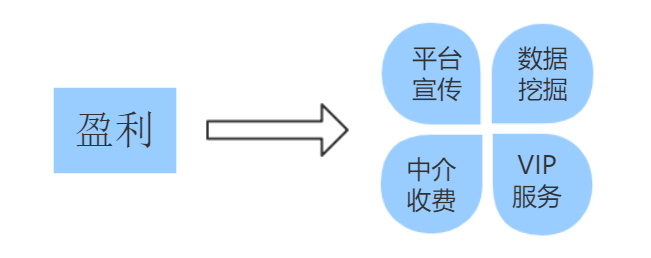
\includegraphics[width=10cm]{fig/1}
	\caption{盈利模式}
\end{figure}

\begin{enumerate}
	\item[(1)] \textbf{平台宣传}
	
	\setlength{\parindent}{2em}发挥平台优势,利用用户宣传效果。一方面,在平台局部适量投放广告,如软件开屏、banner页等。另一方面,为入驻超市商家提供推荐类宣传服务,如菜谱、食物推荐位。
	
	\item[(2)] \textbf{中介平台收费}	
	
	\setlength{\parindent}{2em}在平台成熟后,对于入驻平台的超市等商户,收取一定的平台中介佣金。平台为合作超市带来商业价值的同时,也能实现本公司的盈利。
	
	
	
	\item[(3)] \textbf{数据挖掘}
	
	\setlength{\parindent}{2em}在信息化社会中,数据已经成为必不可少的生产要素之一,合理得掌握并应用数据将为商家带来巨大的价值。而作为饮食推荐服务平台的“食刻Diet”积累了大量的用户数据,将分析大数据所得到的报告卖给商家,将获得丰厚的汇报。
		
	\newpage
	
		
	\item[(4)] \textbf{VIP服务}
		
	\setlength{\parindent}{2em}在平台成熟后,“食刻Diet”平台为用户提供VIP会员服务,用户可享受会员专享受的服务。会员每个月向平台缴纳会员费用。VIP权限包括但不限于,更多菜谱的使用权限、更优先的生鲜订单处理、更迅速的生鲜派送、更多的会员生鲜折扣等等。
\end{enumerate}


%-------------------%
\subsection{营销战略}
运用4C策略来开拓产品市场,以体现我们的创新服务理念和先进服务技术。在市场的营销过程中,顾客是核心,抓住顾客的需求,以服务为重点,考虑顾客的成本,为顾客提供最优的便利,与顾客有效的沟通。

\textbf{线上营销采用新媒体网红IP营销、搜索推广、短视频营销、与APP合作等方式进行推广。}运营自己的产品公众号,写一些饮食相关图文进行推广。在短视频营销上,可以找一些美食博主合作,或者运营独立短视频账号,通过发布一些烹饪、饮食视频来吸引关注,再慢慢渗入平台的推广信息。

\textbf{线下营销可以找一些超市合作,针对目标人群,进行宣传推广。}在超市张贴一些宣传海报,或是设置一些工作人员以奖品吸引人群体验了解。

%%
\subsection{实施运营}
\subsubsection{适时调整}
“食刻diet”电子商务平台的总体定位是:为广大民众打造一款,多功能化饮食攻略平台,让下厨更加简单轻松,让饮食更加合理健康。




	\begin{itemize}
	\item[*] \textbf{平台紧跟用户需求进行调整 }
	
	\setlength{\parindent}{2em}平台的出发点是用户需求。用户口味需求、功能性饮食需求(健身、减脂等)、特殊人群饮食需求(患者、孕妇)决定我们的平台功能块。我们要时刻关注用户群体的需求变化,在平台的搭建维护中不断调整、适应。也需要开放一些意见征集端口,与用户保持密切的沟通联系。		
	
	\item[*] \textbf{确保平台提供信息均符合营养学 }
	
	\setlength{\parindent}{2em}平台搭建的基础是营养学。 平台需要保证,智能算法为用户定制的饮食方案都是健康的;包括膳食结构的衡量、卡路里的计算都是合理的;饮食忌讳的科普知识都是正确的。涉及饮食部分都是相当重要的,平台上的所有发布信息都要慎重、多加筛查。
	
	\item[*] \textbf{为用户提供购买生鲜的评价机制 }
	
	\setlength{\parindent}{2em}用户收到在平台链接购买的生鲜后,可以对收到的生鲜、骑手服务进行评价。若生鲜存在质量问题,可拍下照片向平台投诉,申请超市赔偿。	
\end{itemize}

\newpage

\subsubsection{线下服务}

\begin{figure}[!htb]
	\centering
	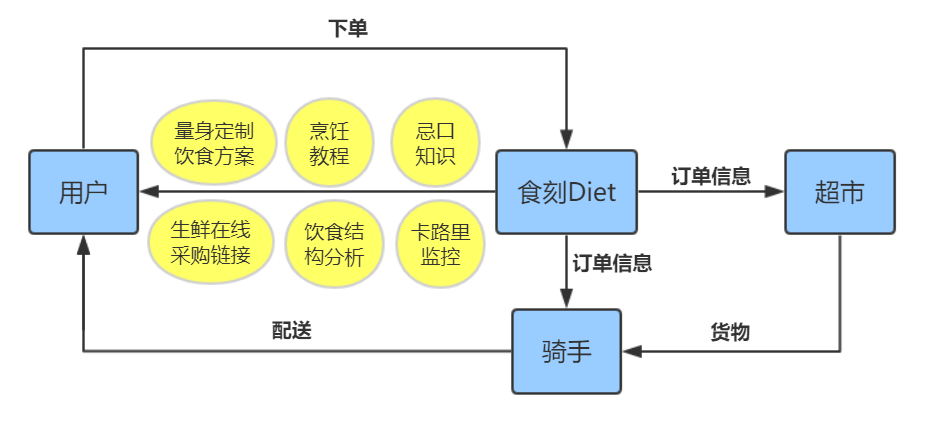
\includegraphics[width=13cm]{fig/2}
	\caption{运营模式}
\end{figure}

	\begin{itemize}
	\item[*] \textbf{与线下超市建立合作 }
	
	\setlength{\parindent}{2em}平台的在线采购生鲜功能,需要线下连锁超市作为供货源。平台需要有超市的生鲜货物信息,包括超市生鲜种类、大致库存、生鲜实物图片,以及生鲜售罄需要在平台同步跟新数据,包括质量问题生鲜的投诉赔偿问题要进行商榷。		
	
	产品初期引进入驻超市,不收取平台费用,后期在平台发展后,开始收取入驻超市佣金。需要再商谈合作细化。 
	
	\item[*] \textbf{线下派送骑手招募 }
	
	\setlength{\parindent}{2em}初期招募骑手标准,要结合初期入驻的超市数量、以及超市辐射范围。对骑手有服务评价机制。
	
	用户在骑手接单后会获得对应的骑手联系方式、骑手所在位置的定位信息,方便随时跟踪订单状态、及时联系骑手。

\end{itemize}


\subsubsection{平台架构}

\begin{figure}[!htb]
	\centering
	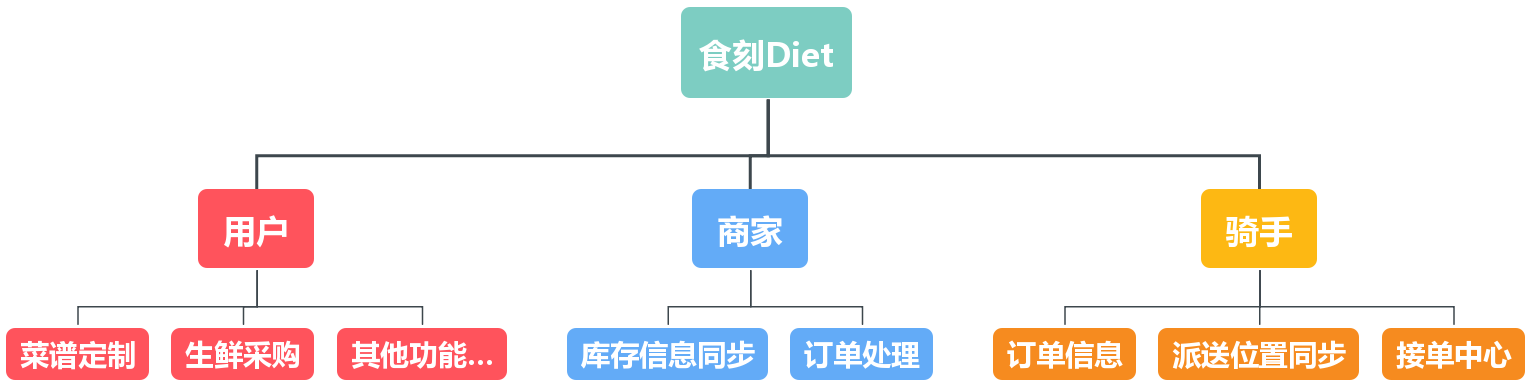
\includegraphics[width=14cm]{fig/pingtaijiagou}
	\caption{平台架构图}
\end{figure}

平台需要有三种界面:用户界面、商家界面、骑手界面。

用户界面相对复杂。有菜谱定制、菜品制作信息检索、生鲜商城、卡路里监控页、摄入营养成分监控页、体系化饮食知识库、饮食圈交流、个人饮食记录等功能块。

商家界面主要功能块是,生鲜库存信息发布、生鲜图片上传,用户订单处理,销量统计,生鲜外送的营业时间设置等。

骑手界面主要功能块是订单处理中心。骑手在订单处理中心接单,获取对应派送订单信息,在派送途中同步自己的定位信息方便用户查看订单所在位置。


\newpage
%---------------------------------------------------------------------------------------------%
\section{市场分析}
%----------%
\subsection{PESTEL分析}
\subsubsection{政策分析(Policy)}
近年来随着我国经济的不断向好各种新兴概念以及产业出现发展,为了维护整个产业环境的稳态发展,我国鼓励并且支持进行互联网产业的创新和发展,李克强从里指出要把以互联网为载体、线上线下互动的新兴消费搞得红红火火,“互联网+”被写入政府工作报告之中。制定行动计划、促进电子商户健康发展、引导互联网产业拓展市场,为了维护市场的健康发展我国更是出台了一系列法律法规及政策文件来维持互联网市场的健康稳态发展。

2015年5月,国务院发布了《国务院关于大力发展电子商务加快培育经济新动力的意见》,提出提出到2020年,基本建成统一开放、竞争有序、诚信守法、安全可靠的电子商务大市场。在支持政策上,《意见》要求为电商企业合理降税减负,逐步将旅游电商、生活服务类电商等相关行业纳入“营改增”范围。降税减负等政策为OMO等新商业模式的成长增添了动力。 

2016年3月,《2016年国务院政府工作报告》提出:聚焦提质增效,推动产业创新升级,制定实施创新驱动发展战略纲要和意见,出台推动大众创业、万众创新政策举措,落实互联网+行动计划增强经济发展新动力。

2017年1月15日国务院办公厅发布《关于促进移动互联网健康有序发展的意见》指出党的十八大以来,党中央高度重视网络安全和信息化工作,成立中央网络安全和信息化领导小组,作出一系列重大决策部署,有力推动了网信事业特别是移动互联网健康发展,对方便人民群众生产生活、促进经济社会发展、维护国家安全发挥了重要作用。

同时针对当前新创建企业,政府同样给予相关支持,文件说明企业要充分运用国家相关政策推动中小微互联网企业在移动互联网领域创新发展,支持和促进大众创业、万众创新,进一步发挥国家中小企业发展基金,国家创新基金等政策性基金引导扶持作用,落实好税费减免政策,在信用担保等服务上予以大力支持,消除阻碍和影响利用移动互联网开展大众创业、万众创新的制度性限制。发展众创、众包、众筹等新模式,拓展境内民间资本和风险资本融资渠道。

2014年国务院国务院印发《关于加快发展体育产业促进体育消费的若干意见》,将全民健身上升为国家战略,2016年《“健康中国2030”规划纲要》成为今后15年推进健康中国建设的行动纲领。国家对全民运动健身的重视,给健身APP行业的发展提供了良好的政治环境,此外,国家对互联网行业发展的支持,并扶持健身行业,也在一定程度上推动了“互联网+运动健身”的进步。

随着经济的发展,人们的收入不断提高,可支配收入占比增大,加上人们对健康的重视,人们越来越愿意为运动健身买单,健身APP的发展有很大的市场空间。此外,大数据、人工智能等技术的进步,资本的加持,也在给健身APP行业不断注入新鲜血液。

\subsubsection{经济分析(Economy)}
根据中国互联网信息中心的统计数据显示,截止2019年6月,中国网民规模已经达到8.54亿人的规模,互联网普及率达到61.2\%。我国网民在二十余年间数量飙升了1400余倍。中国信息通信研究院发布的《中国数字经济发展与就业白皮书(2019年)》指出,经测算,2018年我国数字经济总量达31.3万亿元,占GDP的比重超过三分之一,达34.8\%。除了巨大的人口规模的先天优势,我国先进的硬件设施和建设速度同样也为我国互联网产业的告诉发展提供技术支持。截止2019年6月底我国LTE普及率达到78.3\%,拥有令人难以置信的12.4亿用户。

\begin{figure}[!htb]\label{5}
	\centering
	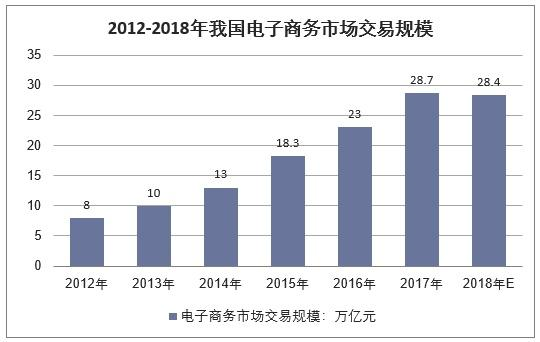
\includegraphics[width=12cm]{fig/5}
	\caption{2012-2018中国电子商务市场交易规模}
\end{figure}

智研咨询发布的《2016-2022年中国电子商务市场分析及未来发展趋势报告》显示2015年中国电子商务市场交易规模为16.4万亿元,增长22.7\%,其中网络购物增长36.2\%,成为推动电子商务市场发展的重要力量。2017年全国年资商务交易额达29.16万亿元,同比增长11.7\%。其中商品、服务类电商交易额21.83万亿元同比增长24\%。




根据中商产业研究院的数据显示,2017全年中国电子商务就业人权达4250万,同比增长13.03\%;琚中商产业研究院预测,到2020年中国电子商务交易额超过40万亿元、网络零售总额达到10万亿元左右、相关从业者超过5000万人。前瞻预计,2019年我国电子商务的交易规模超35万亿元;未来电子商务行业成交规模的增速将有所放缓,到2024年,我国电子商务的成交规模将超过55万亿元。

\subsubsection{社会分析(Social)}
随着我国经济持续快速发展、人民生活水平大幅提高、多元化的电子商务商务服务需求。我国电子商务产业也在不断进行分化提升,电子商务服务市场正经历着结构升级。

根据德勤中国发布的《数字化生活服务市场生态展望报告》,称生活服务领域的数字化超级平台的崛起,将形成新的平台经济,并全面住到生活服务市场。《报告》显示到2023年生活服务市场整日规模将达到3.3万亿元,接近2017年水平的一倍,其中生活服务电子商务市场目前市场规模已达2.7万亿,未来5年有望超过8万亿。随着中国经济形态的不断发展,第三产业也就是服务业将逐渐成为中国社会经济增长的主要引擎。

\begin{figure}[!htb]
	\centering
	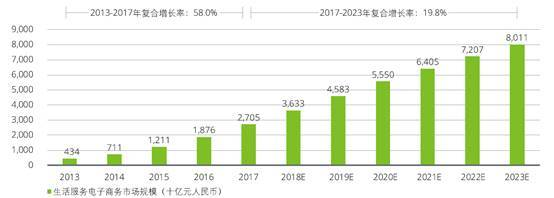
\includegraphics[width=14cm]{fig/3}
	\caption{生活服务电子商务市场增长情况}
\end{figure}

\subsubsection{环境分析(Environmental)}
近年来,在国家大力推进信息化和工业化融合的环境下,我国服务行业、企业加快信息建设步伐,电子商务应用需求变得日益强劲。近年来很多非常传统的行业领域在开展电子商务应用方面取得了较好的成绩。

国内互联网产业市场增长潜力巨大。我国已经进入了全面建设小康社会的阶段,消费结构也进入了全面升级阶段。根据中国互联网信息中心的统计数据显示,截止2019年6月,中国网民规模已经达到8.54亿人的规模,互联网普及率达到61.2\%。我国网民在二十余年间数量飙升了1400余倍。。中国信息通信研究院发布的《中国数字经济发展与就业白皮书(2019年)》指出,经测算,2018年我国数字经济总量达31.3万亿元,占GDP的比重超过三分之一,达34.8\%。除了巨大的人口规模的先天优势,我国先进的硬件设施和建设速度同样也为我国互联网产业的告诉发展提供技术支持。

随着互联网技术、平台、应用、商业模式与移动通信技术紧密结合,移动互联网新技术快速演进、新应用层出不穷、新业态蓬勃发展,工具属性、媒体属性、社交属性日益凸显,生态系统初步形成、加速拓展,越来越成为人们学习、工作、生活的新空间。

\subsubsection{法律分析(Legal)}
自1997年诞生第一家专业电子商务网站以来,中国电子商务产业蓬勃发展。目前已形成B2B,C2B,C2C,O2O等以及第三方支付等多元化发展市场。随着市场法律体系在不断完善,目前我国已经颁布包括电子商务类、网络购物类、电子支付类三大类约三十部相关内容的法律法规。2017年1月15日国务院办公厅发布《关于促进移动互联网健康有序发展的意见》指出党的十八大以来,党中央高度重视网络安全和信息化工作,成立中央网络安全和信息化领导小组,作出一系列重大决策部署,有力推动了网信事业特别是移动互联网健康发展,对方便人民群众生产生活、促进经济社会发展、维护国家安全发挥了重要作用。

2019年1月1日起,《中华人民共和国电子商务法》正式实施,为我国各种新生电子商务模式进行界定,在保护消费者的同时也是为经营者的进行了监管和督促促进电子商务市场的稳态发展。

%----------%
\subsection{行业市场分析}
\subsubsection{知识分析平台市场分析}
2016年被成为中国知识付费元年,根据国家信息中心分享经济研究中心发布的《中国分享经济发展报告2017》,2016年随着得到、知乎live、喜马拉雅FM等知识付费服务商的出现,中国知识付费业态已经找到了新的生长节点。有知识付费意愿的用户暴涨了3倍,知识付费用户达到近5000万人,知识付费新业态正在中国以前所未有的速度崛起,已然成为经济发展各业态的风口。

\begin{figure}[!htb]
	\centering
	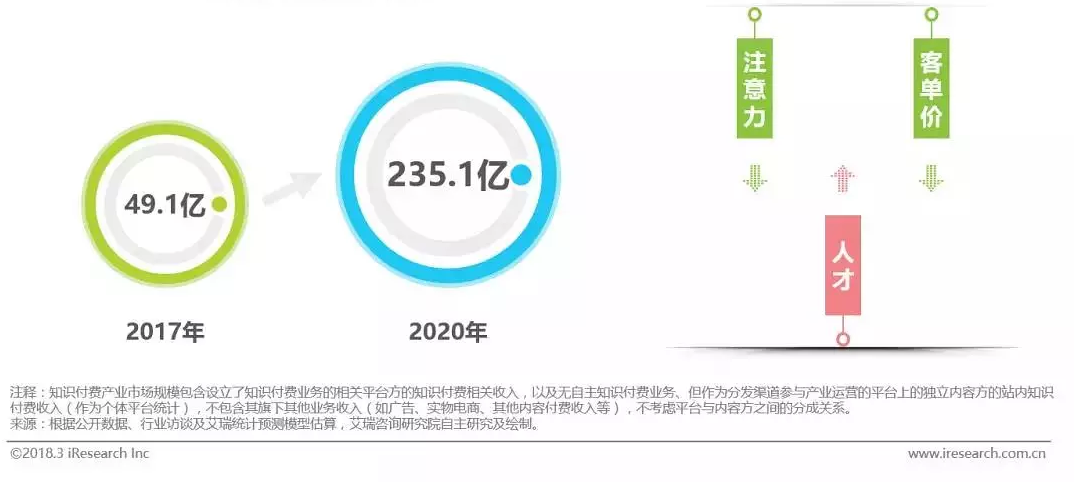
\includegraphics[width=13cm]{fig/6}
	\caption{中国知识付费产业市场规模预测}
\end{figure}



知识付费产业当前形成“腰型”结构,根据数据显示,头部TOP3知识付费平台缠距35\%产业规模,腰部TOP4-10玩家缠距25\%产业规模,此外众多长尾参与者分享其余40\%份额。不同于传统的电子商务平台,由于不同的知识分享产品的目标用户及注重点不同几乎不存在一家独大、头部通吃的局面。
由于知识付费产业的核心动能是用户的明确获知需求,因此在与客户个性化显著的长尾需求相符的前提下,付费率高评价好的产品,均有较大概率进入用户的预购清单。知识付费产业头部格局已经基本形成。未来,综合型、规模化的内容知识付费新玩家将减少,但面向特定领域、场景、用户群的“小而美”的垂直知识付费平台仍有较大发展空间。新小玩家可以通过挖掘垂直领域专精人才、在垂直用户中建立影响力、逐步释放付费潜力,探索领域相关的其他变现模式。

\subsubsection{垂直领域知识分享市场分析}

\begin{figure}[!htb]
	\centering
	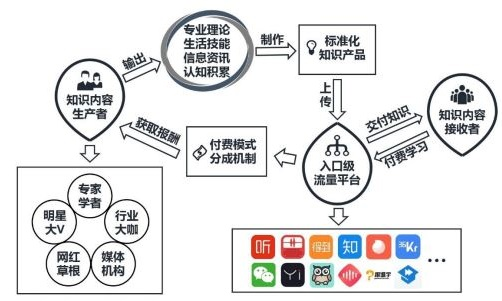
\includegraphics[width=9.5cm]{fig/4}
	\caption{知识付费发展场景}
\end{figure}

知识付费是共享经济的一种主要形式。实际上,知识付费是指知识内容生产与创造者将信息资讯、专业理论、生活技能等有价值的内容进行系统化地加工与梳理进而转化成标准化的知识产品,之后再通过入口级流量平台将其以付费形式传递给用户,以满足用户认知提升、消解焦虑、丰富谈资等各方面需求的业态形式,是泛知识的内容产品化与商业价值的转换过程,是一种以有偿方式传播优质内容的价值交付方式。知识付费自其源起至今,呈现出显著的垂直化与分众化趋势,在这个过程中,恰当的场景构建或许能够成为垂直领域知识付费发展的有效路径。

“为优质内容付费”的消费意愿是在中产阶级崛起的社会背景下产生与发展的,随着互联网技术的升级与传播模式的转变,“人人皆媒”迅速将信息学稀缺转变为信息盈余,于是用户的知识付费需求从根本上发生了转变,用户对知识获取的目的已经从“了解”转向追求“掌握”,寻求神父解决方案的用户对于“一对一”和直接交流的需求空前显现。付费用户在需求测对优质内容更为深度和个性的需求,直接导致了知识付费继续向垂直领域的探索与下沉。



%----------%
\subsection{SWOT分析}
\subsubsection{优势(Strength)}
给予微信小程序来进行内容的发布与展示,用户使用方便快捷。设计简洁清晰,操作简便剋选哪个,服务完善多样。通过数据库技术及云技术将大量的冗余信息进行集合处理。有经验的用户可以通过我们的数据展示来自行安排使用和了解,通过我们的算法技术,即使是没有经验的用户也可以通过我们的个性化功能页面通过自身的情况在系统指引下进行安排。由于国内健身市场并未成熟,人民在健身及饮食安排相关知识欠缺,不一定每个人都有兴趣和时间来进行相应的学习和知识的整理,而我们通过用户自身情况进行个性化安排通过降低用户使用门槛的方式来达到“傻瓜”式的引导。

商业模式上我们通过将新零售概念与知识分享概念进行结合为用户完成消费闭环。在我们的程序上完成从信息上的指导到零售的闭环。
\subsubsection{劣势(Weakness)}
\begin{enumerate}
	\item[(1)] \textbf{前期推广营销有一定的难度 }
	
	\setlength{\parindent}{2em}我们的目标用户是对健康饮食、健身有一定兴趣人群的垂直领域用户,区别与电商企业针对特定群体的产品在推广中只有做到精准投递广告信息才能吸引到用户的使用。所以在企业发展的初期如何吸引到我们的目标用户群体是至关重要的,在着一方面我们存在着较大的问题。
	
	\item[(2)] \textbf{缺少可借鉴的模式 }	
	
	\setlength{\parindent}{2em}我们的产品目的和盈利方式是通过为用户提供个性化的饮食安排和指导来完成用户的消费闭环,通过我们的产品直接下单并进行配送,但是这样的净菜配送服务在我国由于仓储和物流费都很高的现实条件由于高昂的运营费用很难通过自身的资源来完成净菜配送的服务。为了完成此项服务我们的选择是与当前的大型连锁超市平台进行合作与超市方达到共赢的效果,但是由于可参考的模式较少现在的大型连锁超市也可以通过外卖软件来进行购买和配送,还不能够很好的考虑到整个过程的全面性,市场的为止空间与合作方的为止空间较大。

\end{enumerate}

\subsubsection{威胁分析}
\begin{enumerate}
	\item[(1)] \textbf{同类产品的威胁}
	
	在市场上已经存在一些专业的注重减肥健身的软件产品,像轻加健身,薄荷健身等产品,他们已经拥有固定的用户人群和自己的营销方案,包括现在的生鲜新零售产品。这将成为我们最大的威胁之一。对于有一定资源基础的平台来讲如果选择整合该领域的市场将会对本产品带来一定的挑战。
	\item[(2)] \textbf{互联网企业进入门槛低,后进入企业竞争激烈 }
	
	互联网产业的行业门槛低,便于新产品的推出。对于我们的基础功能即健身饮食指导、知识内容分享、以及个性化食谱定制等功能可以通过我们的技术人员的算法及数据库技术和后期运营通过专业人员产生内容来完成。届时的难点在于消费闭环的完成。	
	\item[(3)] \textbf{前期融资与平台合作困难,投资者投机性大 }	
	
	互联网时代以单纯的流量来制造红利的时期已经过去,投资者的选择随着各类产品的丰富趋于理性。而且由于我们的产品的购买环节即净菜配送功能的产品即生鲜菜品基本没有独立运营的能力,我们最好的选择就是通过与大型连锁超市进行合作作为超市方打通线上销售的零一渠道
\end{enumerate}

\subsubsection{机会分析}
\begin{enumerate}
	\item[(1)] \textbf{我国健身人群数量不断上升 }
	
	\setlength{\parindent}{2em}随着人们健康意识的增加,越老越多城市白领人群加入健身运动行列。截止2018年5约,中国健身运动行业月活已经突破6800万人。且健身行业中青年人群占据主体地位。健身运动APP女性用户略多于男性用户;用户中75\%以上为35岁以下年轻群体。由于年轻群体消费观念的升级和消费能力的提升,我国的健身市场还有着巨大的潜力可以探索。
	
	
	\item[(2)] \textbf{国内健身群体相关知识的缺失 }	
	
	\setlength{\parindent}{2em}我国健身人群的数量群体不断扩大,互联网及终端产品的普及以及由于我国的健身文化才处于起步阶段,全民健身环境建立还处于发展阶段,民众普遍对健身知识的了解较少且不愿花费较多的时间进行学习,而为用户直接提供健身知识、指导的健身APP既然收到用户青睐。目前健身APP的月活已经超过7000万人次向亿级人次发展。

\end{enumerate}

\begin{figure}[!htb]
	\centering
	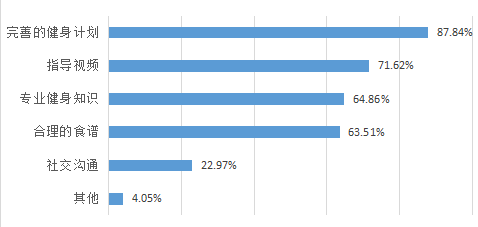
\includegraphics[width=12cm]{fig/7}
	\caption{用户使用健身APP的需求}
\end{figure}

上图数据显示在健身APP的使用人群中,有超过60\%的用户有对专业健身知识的需求和合理的食谱安排。这无疑为我们的发展提供了广阔的空间和机会。

%-----------%

\subsection{中国电子商务发展趋势分析}
中国电子商务电子商务的发展阶段到目前为止经历了三个重要时期,2005年-2010年的流量红利期,2010-2014年的品牌化时期,2015年以后的精细化运营时期。(如图\ref{8})

\begin{figure}[!htb]
	\centering
	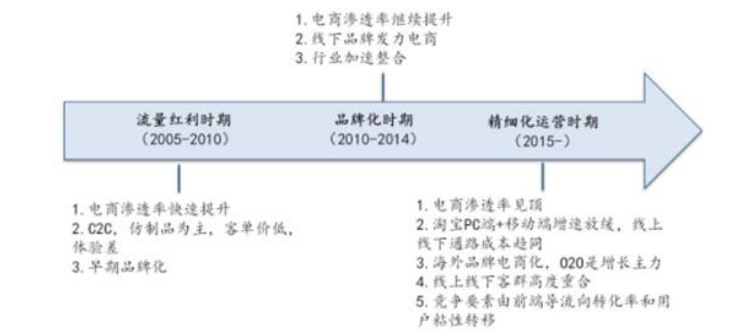
\includegraphics[width=12cm]{fig/8}
	\caption{中国电商发展的阶段}\label{8}
\end{figure}

2018年中国电子商务交易总额31.63万亿元人民币,同比增长8.5%。
该报告从现状规模、发展特点、趋势走向等各方面,多维度对中国电子商务的发展进行了研究和分析。该报告主编、上海理工大学管理学院教授樊重俊称,该报告是反映2018年中国电子商务发展状况的综合性报告,从中可全面了解到中国电子商务的发展水平、发展特点和发展趋势。

从《中国电子商务发展报告2018-2019》报告可见,中国电子商务规模持续扩大,自2016年开始从超高速增长期进入到相对稳定的发展期,但2019年上半年,实物商品网上零售额同比增长仍高达21.6\%,电子商务继续承担国民经济发展的强大源动力。


根据中国互联网信息中心的统计数据显示,截止2019年6月,中国网民规模已经达到8.54亿人的规模,互联网普及率达到61.2\%。我国网民在二十余年间数量飙升了1400余倍。。中国信息通信研究院发布的《中国数字经济发展与就业白皮书(2019年)》指出,经测算,2018年我国数字经济总量达31.3万亿元,占GDP的比重超过三分之一,达34.8\%。除了巨大的人口规模的先天优势,我国先进的硬件设施和建设速度同样也为我国互联网产业的告诉发展提供技术支持。截止2019年6月底我国LTE普及率达到78.3\%,拥有令人难以置信的12.4亿用户。

从中国电子商务从业人员规模来看;2017全年中国电子商务就业人员达4250万人,同比增长13.03\%;2018年中国电子商务就业人员将突破4800万人。


\newpage
%---------------------------------------------------------------------------------------------%
\section{公司竞争力分析}
\subsection{食刻 Diet竞争力分析}
食刻 Diet平台整合了量身定制菜谱、提供菜品烹饪方法、生鲜新零售、卡路里监控、摄入营养成分监控、体系化饮食知识库、饮食圈交流等功能块,功能丰富、实用性强。

不管是只有普通口味需求的用户,还是有瘦身健身功能性需求的用户,抑或是孕妇、患者、婴幼儿等特殊人群,都能在平台得到适合、科学、健康、多样的饮食菜谱推荐。

食刻 Diet平台整合饮食知识库、海量菜品的制作配方、烹调讲解的视频、图文。用户能在平台获取绝大多数所需要的饮食方面的信息。检索、获取获取快捷又便利。


\subsection{主要竞争对手分析}

盒马鲜生是阿里巴巴对线下超市完全重构的新零售业态。盒马既是超市,也是餐饮店,又是菜市场。盒马运用大数据、移动互联、智能物联网、自动化等技术及先进设备,实现人、货、场三者之间的最优化匹配,从供应链、仓储到配送,盒马都有自己的完整物流体系。


盒马鲜生实现用户月购买次数达到4.5次,坪效是传统超市的3-5倍。此外,盒马用户的黏性和线上转化率相当惊,线上订单占比超过50\%,营业半年以上的成熟店铺更是可以达到70\%,而且线上商品转化率高达35\%,远高于传统电商。目前,成熟门店如上海金桥店的线上订单与线下订单比例约为7:3。


\subsection{潜在竞争对手分析}

市场现有大量以用户端分享食谱、健身减肥、生鲜新零售类的公司,此类公司若选择联盟或开发新业务,极有可能会模仿食刻 Diet的运营理念,因此,我们选择这两类公司进行潜在竞争对手分析。

\begin{itemize}
	\item[*] \textbf{与专攻烹饪信息类平台比较}
	
	\setlength{\parindent}{2em}目前市场上有的厨房类APP,以下厨房为例,下厨房自2011年上线运营至今总下载量达4亿次,用户群体基础庞大。下厨房提供大量种食材的图文介绍,包括详细的营养成分、功效、如何挑选、储存方法、适用人群、制作小知识、饮食小知识、相关菜谱等内容,同时提供购买食材服务,但配送周期长,食材新鲜度无法得到保障。为用户提供各色菜品烹饪信息,这和我们的产品有功能重合点,但其缺陷也相对较多。一方面,这些平台只做了一些简单口味的分类,但缺乏健身餐、减肥餐、患者饮食等功能性、特殊性饮食的模块。另一方面,这些APP推荐的只是单一菜品,缺乏多样菜品合理搭配建议,更没有长周期的饮食计划推荐。
	
	\item[*]\textbf{生鲜新零售类平台比较} 
	
	\setlength{\parindent}{2em}市场上既有像每日优鲜等专注配送生鲜的APP,包括美团也有果蔬类外卖板块,而且这些平台运营已经相对成熟。例如每日优鲜,自2014年12月正式成立以来,2017年8月,每日优鲜宣布其单月营收突破2.8亿元,月订单量300万,一线城市全面盈利。仅仅成立三年,每日优鲜已经成为生鲜电商的领跑者。如今腾讯已领投每日优鲜的三轮投资,不仅为每日优鲜带来资本优势,更带来了技术和智慧零售能力的支持。目前微信月活跃用户已达10.4亿,凭借着微信小程序,每日优鲜有着得天独厚的优势。但每日优鲜仍以水果为主要品类,高频刚需引流作用明显,主营业务仍为食材原料配送。我们的“食刻Diet”也有生鲜配新零售功能块。但我们的平台与这些主打生鲜新零售的电商平台定位不同。
	
	“食刻Diet”主推功能是,针对用户需求量身定制健康饮食方案,提供菜品烹饪信息,并对摄入卡路里、营养成分进行监控。建立的生鲜商城,选定菜谱后的一键式采购生鲜,也都是为用户下厨更加方便快捷而设定。
	
	\item[*]\textbf{与健身减肥类平台比较}
	
	\setlength{\parindent}{2em}目前市场上有注重健身、减肥类的APP,例如薄荷APP,里面的功能性饮食菜谱推荐、卡路里检测与我们的产品有部分的重合之处。
	
	但从定位而言,这类APP专攻瘦身健身的功能性饮食,而我们的产品不仅仅满足这一部分群体需求,还满足更多普通用户的长期饮食定制。其次,我们的产品不仅仅只进行卡路里摄入的监控,还对碳水化合物、蛋白质、脂肪等摄入结构进行监控,并在摄入架构不合理时对用户进行提醒、推送平衡摄入的相应菜谱建议。
	
\end{itemize}

\subsection{波特五力分析}

利用麦可·波特提出的五力分析架构(如图\ref{wuli})对“食刻Diet”产品方案进行分析。

\begin{figure}[!htb]
	\centering
	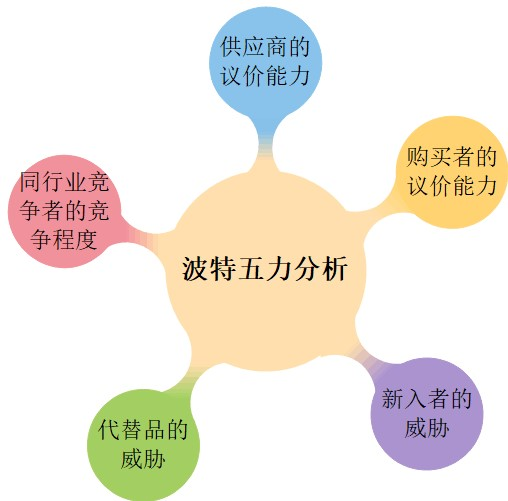
\includegraphics[width=9cm]{fig/botewuli}
	\caption{波特五力分析图}\label{wuli}
\end{figure}

\subsubsection{供应商的议价能力}
 “食刻Diet”的对接超市选择范围广,食谱对应料理的多数食材均为日常食材,食材成本较低,因此普通食材超市端的议价能力较弱;如果消费者选择少数的高阶食谱或者偏好有机食材,对于此类高档食材,一般的超市不会进货,对应的高端食材店铺的议价能力相对较高。
 
\subsubsection{购买者的议价能力}
当市场有多款类似服务的公司时,消费者会出现比价心理,特别是目前生鲜配送行业的迅猛发展,会给本公司产品定价造成一定影响。从此种意义上说,时间充裕消费者议价能力较强。

对于忙碌的都市工作者,她们更倾向于花费更多的金钱,选择更到位的服务,对于这部分消费者来说,她们的议价能力较弱。

鉴于存在同类商品的竞争,公司可以采取的策略是结合成本制定合理的定价策略、同时也要制定一系列优惠策略,比如在“双十一”、“双十二”时采取薄利多销的方法,打折出售商品;给老用户赠送免费配送卷等活动巩固已有客户。而长远的策略是通过提供更新鲜的食材,更健康的饮食食谱和健康理念吸引消费者,通过品牌核心竞争力取得市场占有率,成为消费者的首选。

\subsubsection{新进入者的威胁}
目前市场的威胁更多集中于单独生鲜配送平台和饮食定制APP,将两者相联系并集合食谱配送的公司并不多见。但是正是由于目前生鲜电商的迅速发展,日后如果这类公司在当前生鲜配送的基础上加入更多服务功能,对“食刻Diet”公司的威胁也十分巨大。

当前生鲜领域,阿里已经在转型,正在尝试跨过生鲜电商,直接进入”新零售生鲜“时代,直接跨入不需要搭建传统物流的三维下半身新零售时代。比如盒马,淘宝便利店和安鲜达的前置仓尝试,三江、银泰的收购,百联的合作等等,以后也会越来越多。

所以,作为新兴领域的“食刻Diet”应该在行业市场还未完全被占领时大力发展用户群体,采取多样化宣传手段,同时保证食材质量,打造行业口碑,积累用户。

\subsubsection{替代品的威胁}
目前国内尚未出现成熟的健康食谱一键式购齐电商平台,食刻 Diet作为微信小程序,操作简单,无需下载APP;并且用户在食刻 Diet建立自己的饮食圈,和朋友分享,食刻 Diet同样支持并鼓励用户在“食刻 Diet内进行视频或文字等各种形式的互动社交。这将增大用户的粘性,而人们对社交性的依赖决定了用户不会轻易放弃食刻 Diet,这就决定了相对于其他APP,食刻 Diet的替代品威胁性较小。

\subsubsection{同行业竞争者的竞争程度}

随着盒马鲜生背后阿里系的大量资本注入,其发展注定更加迅速。但是尾大不掉,盒马鲜生主打的现场制作背后也呈现出大量问题,员工态度不佳,食材问题屡屡出现。食刻公司市场占有率和知名度虽然不及盒马鲜生,但是可以借鉴盒马鲜生的经验,努力做好品控,为用户提供最新鲜的食材,最美味的食谱,优质的服务与独特的商业模式不仅能提高品牌的知名度,也能扩大市场范围。


\newpage
%---------------------------------------------------------------------------------------------%
\section{创新策划方案介绍}
%------------%
\subsection{小程序综述}
食刻 Diet是服务于健康食品市场的,以用户订购食材并进行配送为核心,强调用户饮食私人化定制的一站式的食品销售平台。小程序提供了C2B与OMO购物平台等多方位的服务,注重用户的体验式营销,提供了饮食记录、分享,健康计划,健康统计与分析,食材配送等新颖功能。小程序以客户为中心,以用户的追求健康的心理为出发点,依靠产品设计中对用户体验的极致追求,提供一套完整的饮食记录与定制,食材采购的方案,帮助用户彻底解决生活中最重要的饮食健康问题。

食刻 Diet基于微信小程序,是一种无需下载安装即可使用的应用,能以最低成本触达用户,对于用户来说,微信小程序UI和操作流程会更统一,这也会降低用户的使用难度。微信搜索页面还有小程序的快捷入口,为常用的小程序带来更多的曝光和开启机会,微信应用号本身是网页,可以在群里被转发,可以搭建到公众号商,传播起来非常方便。商家可以通过更多的渠道来推广自己的小程序,进而实现店铺及商品的推广交易。并且,小程序可以大大降低运营成本,对创业者还是传统商家来说都是一大优势。

\textbf{小程序名称:}食刻 Diet

\textbf{服务对象:}对饮食方面了解较少,不愿耗费时间规划饮食、采购食材者但又想追求健康饮食的群体

\textbf{小程序类型:}C2B+OMO电子商务平台

\textbf{小程序目的:}专注于健康饮食规划领域,为日益增多的广大用户解决了食材采购,饮食规划的问题,提供一站式全方位服务。促进超市食材促销、促进健身文化发展、有利于人民健康生活水平的提高。

%------------%
\subsection{小程序特色}

\begin{figure}[!htb]
	\centering
	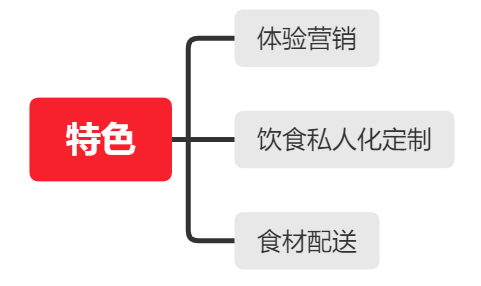
\includegraphics[width=10cm]{fig/18}
	\caption{食刻 Diet小程序特色图}
\end{figure}

通过解决用户在饮食方面的一系列问题吸引用户,以用户成长+饮食成长绑定用户,以个性化饮食定制及食材配送为用户提供全方位、多样化的服务,真正解决用户烦恼,提升用户的健康生活水平。

\newpage
%------------%
\subsection{小程序整体功能}
\begin{enumerate}
	
	\item 用户使用流程
	\begin{figure}[!htb]
		\centering
		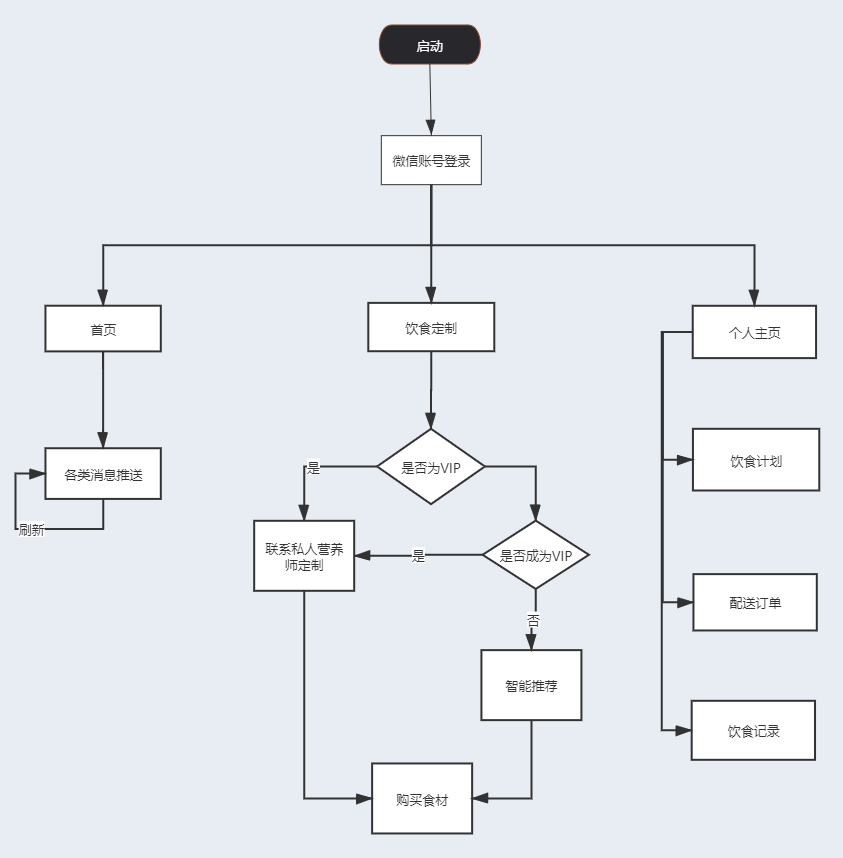
\includegraphics[width=14cm]{fig/19}
		\caption{用户使用流程}
	\end{figure}
	
	\newpage
	
	\item 功能解析	
	\begin{figure}[!htb]
		\centering
		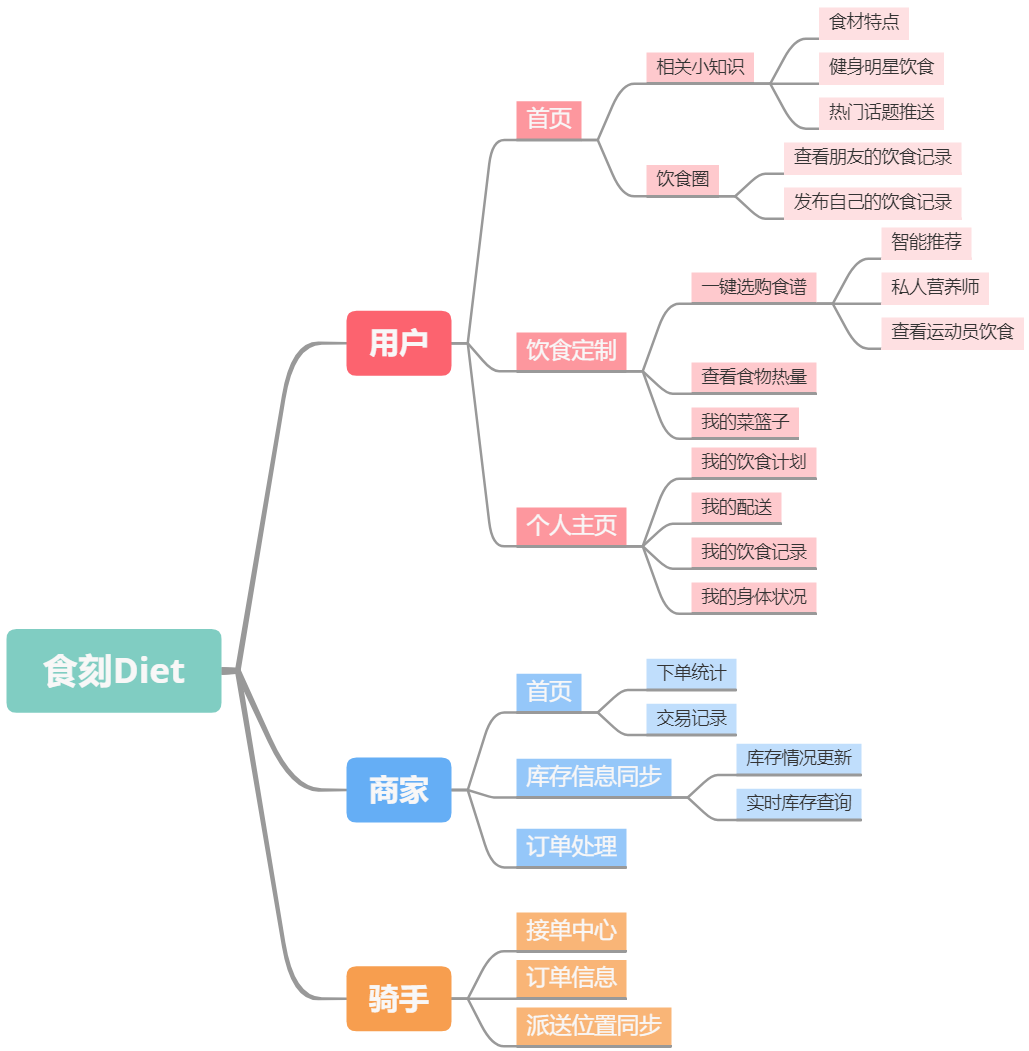
\includegraphics[width=14cm]{fig/Diet}
		\caption{小程序功能示意图}
	\end{figure}
	
	
	
\end{enumerate}


%------------%
\subsection{ 微信 C2B + OMO 解决方案}
\subsubsection{C2B+OMO解决方案设想}

C2B(Consumer to Business,即消费者到企业)是先有消费者需求而后有企业生产,作为互联网经济时代新的商业模式,改变了原有生产者(企业和机构)和消费者的关系。即先有消费者提出需求,后有生产企业按需求组织生产。通常情况为消费者根据自身需求定制产品和价格,或主动参与产品设计、生产和定价,产品、价格等彰显消费者的个性化需求,生产企业进行定制化生产。C2B的核心是以消费者为中心,消费者当家做主。平台优选使用的产地直采模式是一种全新的生鲜电商供应链模式。客户通过网上商城下单,在超市的员工进行采购,有效地精简整个流程。同时,平台与多家生鲜、农场产地合作。这一模式在后续进行的OMO模式中也继续使用。

“C2B”模式之所以成为很多企业发展新模式的探索,究其原因是其恰逢其时地迎合了80、90后新生代消费群体的内心需求。对于超市商家而言,它的推出有助于商家更加精准地锁定消费者,提前备货,减少库存,更有效地管理上下游供应链,更精准地提供消费者需要的服务形式。

OMO模式相比于之前的B2C和C2B以及O2O模式,最大的优势与特色就是在满足顾客线上消费的前提下,最大限度地提升顾客门店的体验。要能收集每个消费者背后庞大的消费行为数据,零售品牌企业则必需跟着消费者的足迹,朝向「OMO虚实融合」,以人为核心去布建全通路经营(Omni Channel) 与销售服务环境,累积更多消费数据,才能做到更加精准的分析与沟通,掌握圈粉策略。眼下比较火热的OMO就是以这样的模式为中国超市企业的未来发展提供了一种便捷可操控的运营方式,也为传统超市配送行业带来了一种全新的营销思维,给超市企业寻求电子商务发展提供了指向标。

由于科技快速发展,在2017年由创新工场的CEO李开复首先提出新零售模式OMO虚实整合这个概念,即借着从线上的行销活动寻找消费者,再将其延伸至线下的一种导流量的模式。因为O2O这种商业营销模式,只是掌握人潮的汇流,却无法做到分众的行销模式,因此衍生出OMO虚实融合(Online Merge Offline/ Offline Merge Online)的概念,在此概念下,线上与线下将相互导流,企业若能模糊实体、虚拟通路与物流管道间的界线,并掌握强大的消费者数据,将有助于企业迈向OMO精准行销的时代。

\subsubsection{食刻 Diet小程序应用能力分析}
\begin{enumerate}
	\item[(1)]在小程序平台上,用户可以以微信为平台的进入接口,实现便捷的小程序实用。
	
	\item[(2)]在小程序上购买商品的用户,可以通过多种方式快捷地实现支付功能。包括有第三方支付(微信等)、网银支付、货到付款等。	
	
	\item[(3)]本平台的数据以及微信用户的LBS等数据可以供平台进行各类数据的交叉分析,对使用小程序的用户进行智能推荐,围绕用户需求,解决用户困惑。
	
	\item[(4)]通过用户端口、微信小程序账号、支付方式、智能分析,将实现本平台在微信小程序端口的完整功能,提供一站式服务。
	
\end{enumerate}

%------------%
\subsection{小程序维护}

微信现在几乎每周都在开放新功能,小程序肯定需要不断地更新迭代,也需要专人维护。小程序不进行后期的维护,就如买手机要摒弃售后服务一样。时间一久,小程序就徒剩一个空壳子,前期小程序开发所做的投资与努力都会付诸东流。而小程序的维护,不单单是指技术数据上的更新,更是指内容上的更新,意即软硬件都要实时更新换代。

就技术而言,小程序要定期修复漏洞,更新版本,否则小程序运行就会出现卡顿,甚至无法运行的问题。再者,若服务器受到攻击,也需及时处理,或者为适应实际情况的需要,对页面以及相关数据进行改动,都需要专业人员进行处理。

就内容而言,该小程序是一款主打便食材配送及健身食谱制定的平台,目前涉及社区互动,食谱推荐及定制以及健身计划记录等内容。而若是提供的内容一成不变,渐渐的该小程序对于受众的吸引力就会减弱,正如市场进行的优胜劣汰一样的道理,逆水行舟,不进则退。所以,小程序要想在业内始终占有一席之地,要将创新精神融入到小程序的维护工作当中去。

因此,我们小程序的维护包括查看留言版,页面更新与布局、数据库维护。


\subsubsection{查看留言板}
通常用户会利用留言板来反映小程序中存在的问题,小程序管理员对这些问题应立即检查,如确实是服务器和页面方面的原因,应及时改善。用户也会对小程序的内容和页面布局提出一些有用的建议,作为管理员应该听取好的建议,从善如流,并把好的建议在今后的小程序更新过程中实施。另外用户会想通过留言板向管理员提出一些问题,管理员应该对这些问题及时回答,并且公布在“查看用户留言”的页面中,以答疑解惑。

\subsubsection{页面内容的更新与布局}
小程序发布后不能总是一成不变,否则经过一段时间后,其中的信息对用户已没有新意,不能吸引到新的用户,并且还会失去一些现有的用户,这样访问数量肯定会减少。小程序更新最有用的依据是系统的日志记录。通过分析用户对服务器资源的访问情况,确定小程序页面内容的增加、删除、修改。

内容更新是小程序维护过程中的一个瓶颈。平台从以下几个方面入手,使网站能长期顺利地运转。

\subsubsection{数据库维护}
开发者可以使用云开发来开发微信小程序,无需搭建服务器,即可使用云端能力。云开发为开发者提供完整的云端支持,弱化后端和运维概念,无需搭建服务器,使用平台提供的 API 进行核心业务开发,即可实现快速上线和迭代,同时这一能力,同开发者已经使用的云服务相互兼容,并不互斥。

目前提供三大基础能力支持:
\begin{enumerate}
	\item 云函数:在云端运行的代码,微信私有协议天然鉴权,开发者只需编写自身业务逻辑代码。
	
	\item 数据库:一个既可在小程序前端操作,也能在云函数中读写的 JSON 数据库。
	
	\item 存储:在小程序前端直接上传/下载云端文件,在云开发控制台可视化管理。
	
\end{enumerate}

后台管理和Web API层是分开的,它们的数据最终都是集中在一个数据库上,实现我们所要的数据集中化管理。微信小程序为我们提供了便捷的云开发模式,无需自己实现鉴权,对接第三方存储。数据方面,增删查改功能非常方便。云开发提供的种种便利,我们优先选择小程序+云开发的方式去实现。

%------------%
\subsection{ 小程序安全及防护措施}
\subsubsection{ 小程序的安全隐患}

由于使用 WebView 和 JSSDK 的人越来越多,微信上越来越多干坏事的人,有人做假红包,有人诱导分享,有伪造一些官方活动,他们会利用 JSSDK 的分享能力变相的去裂变分享到各个群或者朋友圈。

由于 JSSDK 是根据域名来赋予 api 权限的,运营人员封了一个域名后,他们立马用别的域名又继续做坏,注册一个新的域名的成本是很低的。

开发者的后台就拿到了前边wx.login()所生成的微信登录凭证code,此时就可以拿这个code到微信服务器换取微信用户身份。微信服务器为了确保拿code过来换取身份信息的人就是刚刚对应的小程序开发者,到微信服务器的请求要同时带上AppId和AppSecret。

AppId和AppSecret是微信鉴别开发者身份的重要信息,AppId是公开信息,泄露AppId不会带来安全风险,但是AppSecret是开发者的隐私数据不应该泄露,开发者需要好好保护。

\subsubsection{小程序的安全措施}

为了保证小程序的质量,以及符合相关的规范,小程序的发布是需要经过审核的。经过审核的小程序才能对外发布,同时在出现问题时,小程序会被下架停用。

另外,每个微信小程序需要事先设置一个通讯域名,小程序只可以跟指定的域名与进行网络通信,包括普通 HTTPS 请求、上传文件、下载文件和 WebSocket 通信。这些通讯域名,也都必须要求通过备案。
同时,小程序必须使用 HTTPS 发起网络请求。请求时系统会对服务器域名使用的 HTTPS 证书进行校验,如果校验失败,则请求不能成功发起。

这些种种的限制和管理模式,都进一步保障了用户的数据和隐私安全。


%------------%
\subsection{小程序开发周期}

\subsubsection{制定计划}
在小程序开发之前,首先应当制定项目开发计划,这是第一阶段,其主要任务如下:
\begin{enumerate}
	\item[(1)]确定要开发项目的目的、目标
	
	\item[(2)]给出功能、设计等方面的要求
	
	\item[(3)]估计可以使用的网络资源,人力资源,开发进度计划,成本和效益
	
	\item[(4)]制定出完整的开发计划,并且发给项目负责人,程序员,美工
	
\end{enumerate}


\subsubsection{需求分析和定义}
根据小程序功能定义进行需求定义,确定网站需要完成的功能。

\subsubsection{小程序设计阶段}
概要设计:把各项需求转为小程序的总体结构和数据结构,结构中每一部分都是意义明确的模块,每个模块都和需求相对应。

详细设计:对每个模块的工作过程给予具体描述。

美工设计:根据详细、概要设计,确定功能,并做出页面设计。

\subsubsection{程序编写}
根据小程序页面设计图纸,在微信开发者工具中变成编程实现。我们用微信小程序专用的JSON数据格式、WXML模板、WXSS样式以及JS逻辑交互。

我们使用小程序+云开发模式,简化小程序后端维护的任务量。云开发模式为我们提供了后端维护的极大便利。

\subsubsection{小程序测试}
我们根据小程序的特点,安置一下测试点:
授权:目前已实现静默授权,即用户首次访问小程序,主动获取微信授权,通过获取openid,生成转转uid,并存储昵称、头像等信息。后续用户若卸载小程序重新进入,无需重新授权。
分享到好友列表\&生成海报页分享到朋友圈
用线上/测试/开发版分享给好友,落地页就是相应的线上/测试/开发版;
朋友圈识别跳转都是线上版;所以在测试过程中若涉及到扫码跳转,就需借助【小程序码测试工具】。
微信版本:小程序的接口完全依赖于微信,因此部分基础库较高的接口可能在低版本的微信上不生效,需做兼容。

不同机型:如某页面在华为机型展示没问题,但到小米机型却展示有问题。
手机系统:Android和ios两个版本兼容性可能不同

\subsubsection{小程序运行维护}
小程序维护有4中类型,它们分别完成以下任务:
\begin{enumerate}
	\item[(1)]纠正性维护:运行过程中发现错误并进行修改
	
	\item[(2)]适应性维护:适应变化的工作环境,做出适当的变更
	
	\item[(3)]完善性维护:增强网站的功能而做出的修改
	
	\item[(4)]预防性维护:为未来的修改和调整奠定更好的基础而进行的工作
	
\end{enumerate}

%------------%
\subsection{小程序开发技术}

云开发是微信团队和腾讯云联合打造的一个“应用服务中台”,整合了微信公众平台和腾讯云的核心技术,能够提供云数据库、云存储、云函数、日志和监控等开发运维能力。通过“小程序·云开发”,开发者可以无缝安全调用小程序的开放服务,提升开发效率,快速试错和落地产品。

云开发主要具备以下四点能力:

云函数:在云端运行代码,微信私有协议天然鉴权,开发者只需专注于编写自己的业务逻辑代码。

数据库:一个既可以在小程序前端操作,也能在云函数中读写的JSON数据库,不再受限于关系型数据库复杂的操作模式构建,数据管理上非常简洁。

存储管理:提供上传文件到云端、带权限管理的云端下载能力,在小程序前端直接上传/下载云端文件,在云开发控制台可视化管理。

部署扩容:因地制宜,开发者在开发工具内编写好代码之后、一键上传部署即可运行发布,快速扩容/缩容。

%------------%
\subsection{法律声明}

法律声明:

食刻 Diet提醒您:在使用食刻 Diet各项服务前,请您务必仔细阅读并透彻理解本声明。您若要访问和使用食刻 Diet,必须不加修改地完全接受本协议中所包含的条款、条件,并且遵守有关小程序及/或本小程序的相关法律、规定与规则。一旦您访问、使用了食刻 Diet,即表示您同意并接受了所有该等条款、条件及通告。

免责声明:

食刻 Diet在此特别声明对如下事宜不承担任何法律责任:

\begin{enumerate}
	\item[(1)]食刻 Diet在此声明,除公司自己公布和上传的信息外,不对任何连接到本网站的信息、广告、站点做出保证和承担法律责任
	
	\item[(2)]拥有公司签约的店家或者会员自行上传的信息,需遵守签约协议,对违反协议而散播不真实、不合法信息者责任自负,公司不承担连带责任
	
	\item[(3)]未经本公司同意与顾客擅自签订协议而发生纠纷者,由双发自行处理,本公司不承担任何责任
	
\end{enumerate}

责任追究声明:

若超市公司与顾客在服务的过程中发生财务或是安全纠纷,由双方自行处理,本公司不承担任何法律责任。

知识产权声明:

\begin{enumerate}
	\item[(1)]食刻 Diet拥有本小程序内所有信息内容的版权	
	\item[(2)]任何被授权的浏览、复制、打印和传播属于本网站内信息内容都不得用于商业目的且所有信息内容及其任何部分的使用都必须包括此版权声明。	
	\item[(3)]食刻 Diet所有的产品、技术与所有程序均属于食刻 Diet知识产权。食刻 Diet其他产品服务名称及相关图形、标识等为食刻 Diet的注册商标
	未经食刻 Diet许可,任何人不得擅自(包括但不限于:以非法的方式复制、传播、展示、镜像、上载、下载)使用。否则,食刻 Diet将依法追究法律责任。
	\item[(4)]所有的权利均在全世界范围内受到法律保护,除非有其他的标注或在此等条款和规则中被允许使用,本网站上可阅读和可见的所有资料都受到知识产权法的保护。
	
\end{enumerate}


\newpage

%---------------------------------------------------------------------------------------------%
\section{页面结构}

\subsection{总体架构}


\begin{figure}[H]
	\centering
	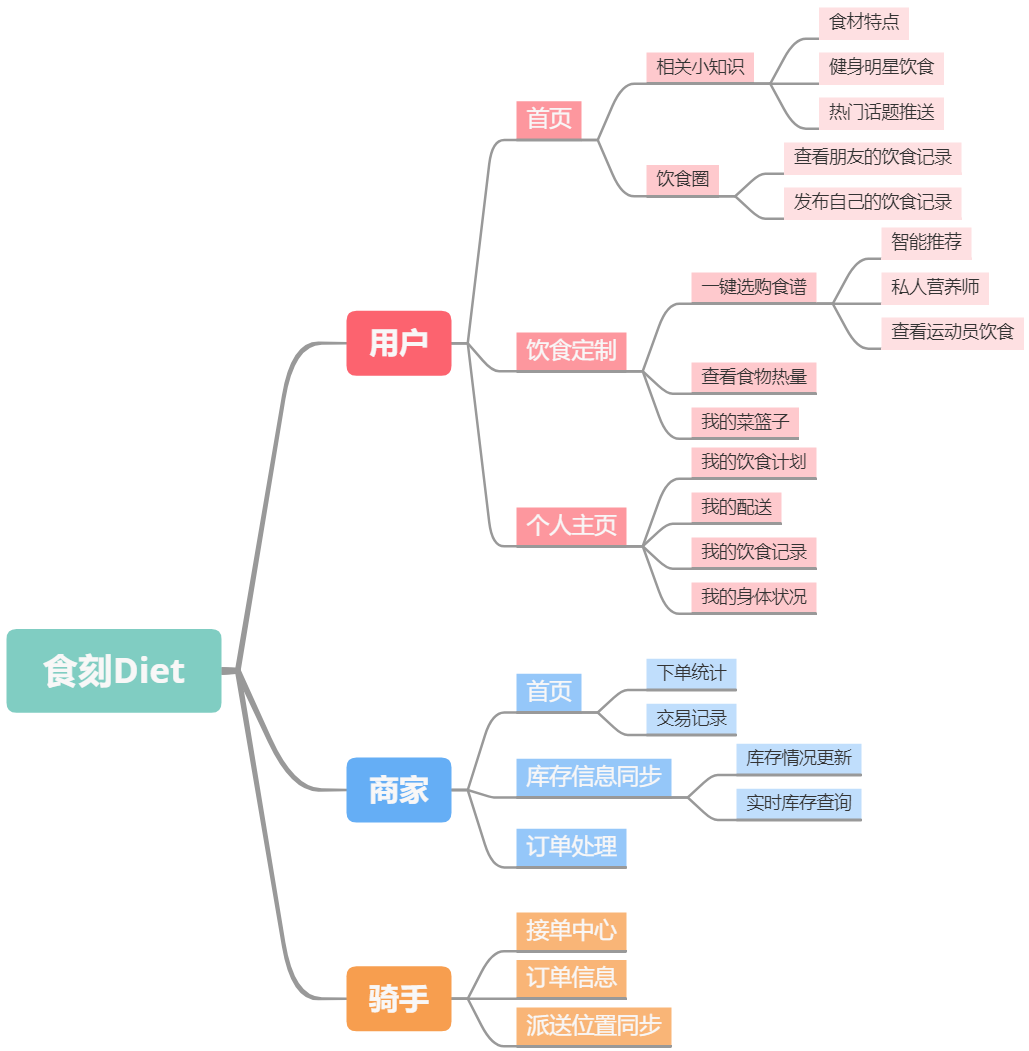
\includegraphics[width=14cm]{fig/Diet}
\end{figure}	

\newpage

\subsection{小程序风格及页面设计}
食刻 Diet的页面风格追求简约、实用、不浮夸,主色调清新。用户在页面中能及时收到个性化饮食相关知识分享,其他用户的饮食记录,并很好的展现出饮食定制计划及完成情况,并对计划提出评价。页面布局清晰,页面跳转设置合理,方便用户使用,提升用户体验感。页面都将以操作方便实用,视觉简约为原则,并能够很好的实现各模块的功能。

\subsection{用户界面}

\subsubsection{一级页面架构}

\begin{itemize}	
	
	
	\newpage
	\item\textbf{微信登陆页面}
	
	\begin{figure}[!htb]
		\centering
		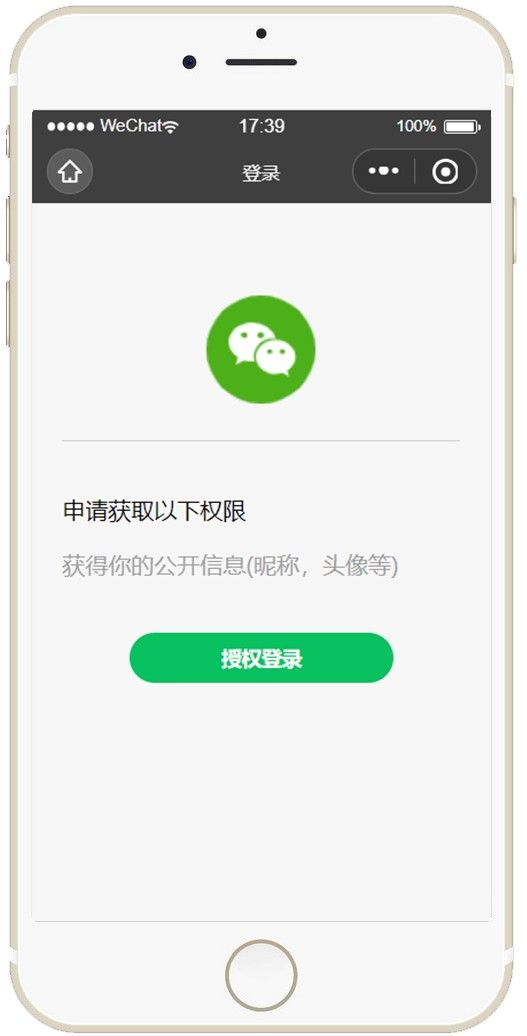
\includegraphics[width=10cm]{fig/!14}
	\end{figure}
	
	\newpage
	
	\item\textbf{首页} 
	
	\parpic{%
		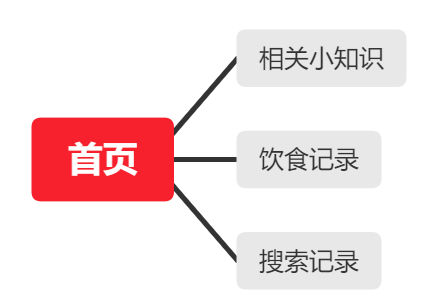
\includegraphics[width=6cm]{fig/31}}
	
	\setlength{\parindent}{2em}小程序的首页是用户进入小程序的第一个页面,这对于吸引用户来说至关重要。因此,我们的首页以内容驱动为主,为游客提供精选的食材相关的新鲜有趣的推送,包括每种食材的特点、健身明星的饮食表、热门话题推荐和当下用户发布的饮食记录等。用游客感兴趣的话题吸引他们,促使更多的游客加入。
	
	\setlength{\parindent}{2em}此外,我们在首页放置导航栏,用户可以通过导航栏快速跳转至其他页面,如普通用户的智能饮食推荐。增加搜索功能,可根据自己感兴趣的关键字搜索饮食相关问题。
	
	\newpage
	
	\begin{figure}[!htb]
		\centering
		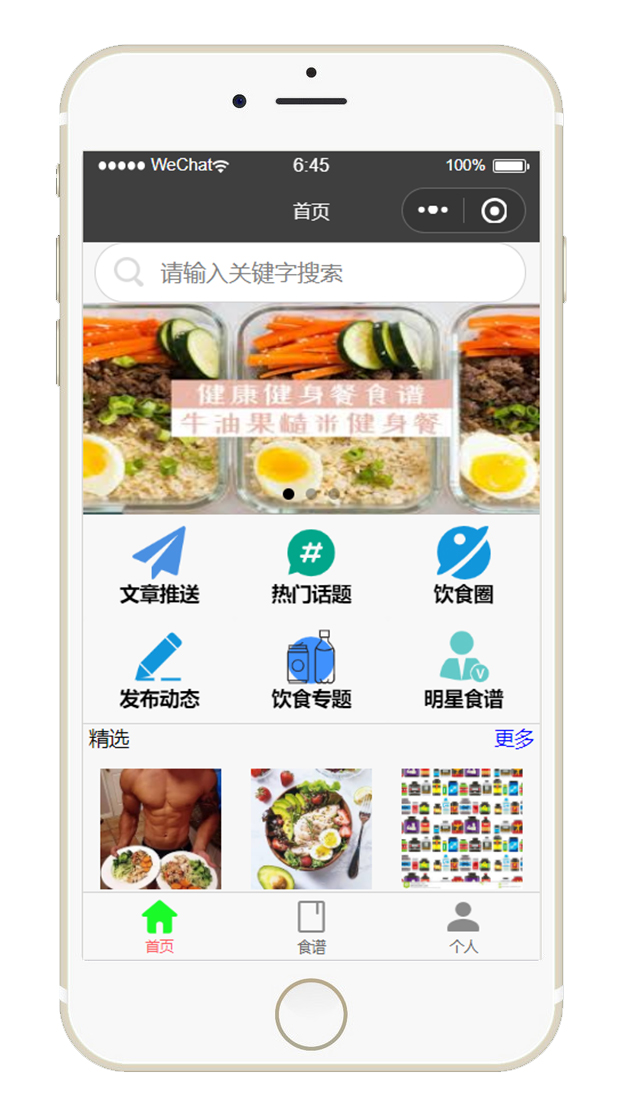
\includegraphics[width=11cm]{fig/!1}
	\end{figure}
	
	
	\newpage
	
	\item\textbf{饮食定制页}
	
	\parpic{%
		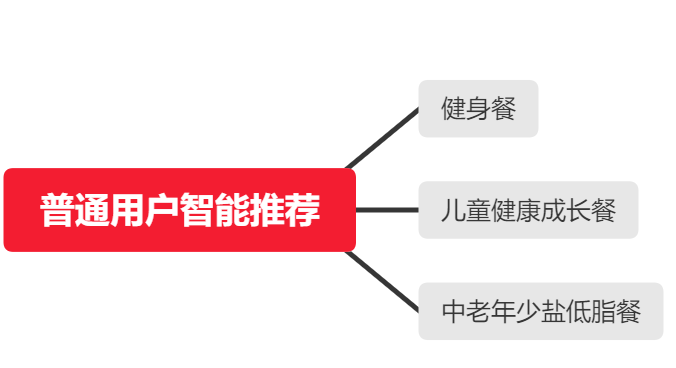
\includegraphics[width=7.5cm]{fig/34}}
	
	饮食定制是本平台的核心功能之一,因此具有较为庞大的结构。并且还要对普通用户和VIP用户进行区分,进一步促进线上消费,
	
	我们将饮食定制分为两部分,一部分为普通用户的智能饮食推荐,推荐较为简单,分为增肌餐、减脂餐两类,用户可根据自己的情况进行选择。
	
	我们给普通用户提供一些智能推荐以吸引他们成为VIP用户。成为VIP用户需要定期支付一定的会员费用,VIP用户可以享受许多更好的服务,可以定制食谱、有私人营养师推荐、查看运动员饮食,自定义饮食计划。
	
	在用户进行选择后,我们将指定的食材加入购物车,核算清单,在用户确定后进行食材配送。
	
	\newpage
	
	\begin{figure}[!htb]
		\centering
		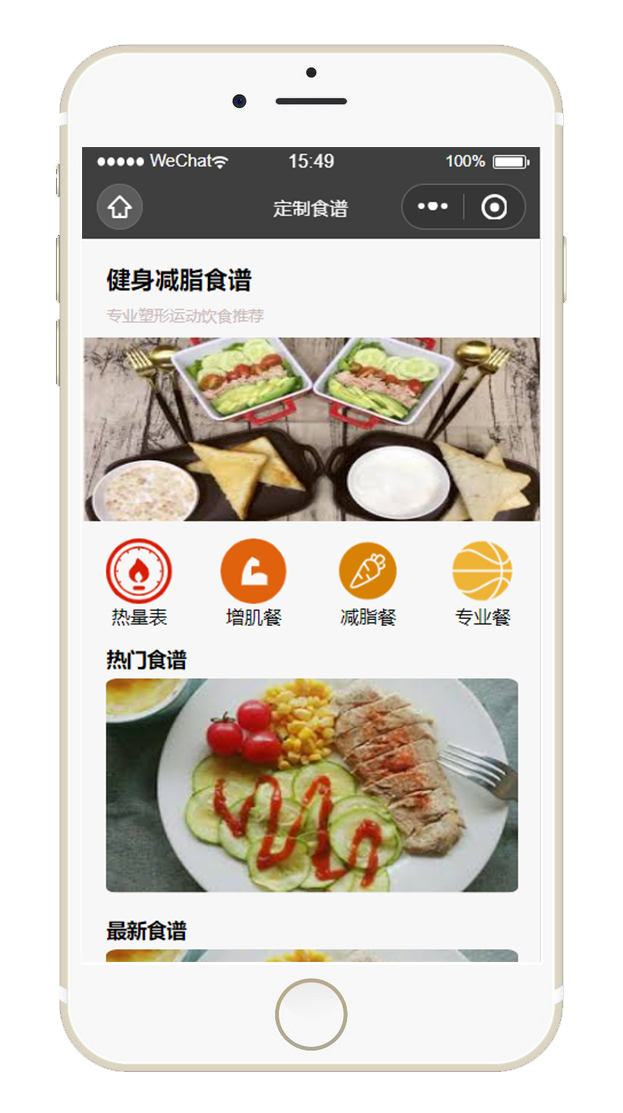
\includegraphics[width=11cm]{fig/!15}
	\end{figure}
	
	\newpage
	
	\item\textbf{个人主页}
	
	对于未注册的游客,我们请求游客使用微信账号登陆。而对于已登陆注册的游客,我们首先在最顶部显示用户的头像,然后在头像下方的导航栏中提供我的身体状况、我的饮食计划、我的配送、我的饮食记录四个主要同级模块。还有一些小模块,例如我的收藏等。用户可点击进入其中一个模块进行相关操作。
	
	\begin{figure}[!htb]
		\centering
		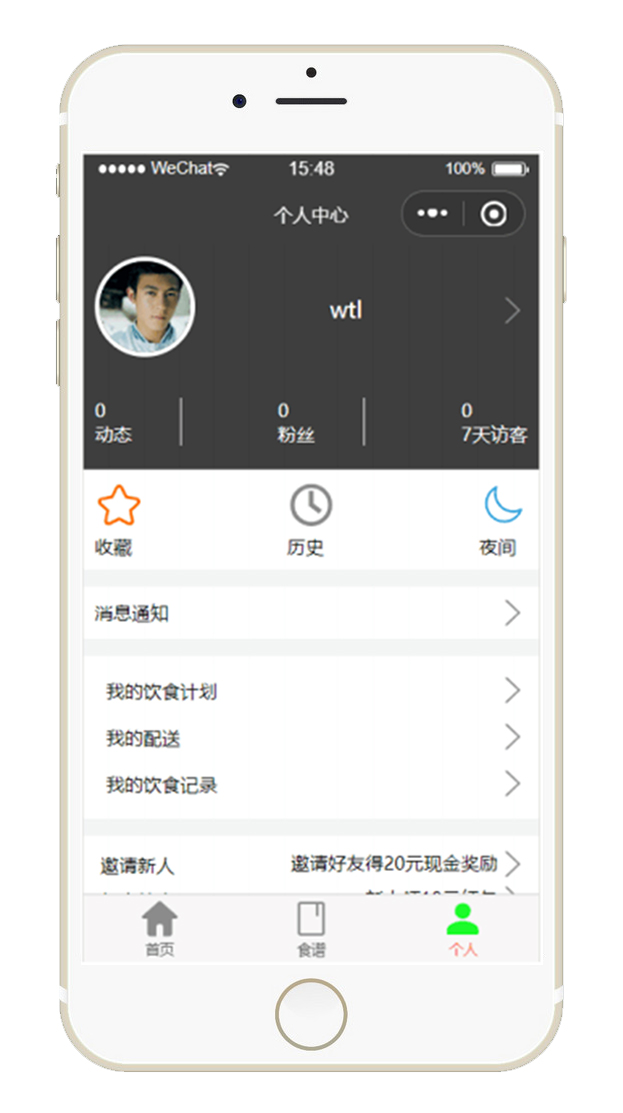
\includegraphics[width=9cm]{fig/!16}
	\end{figure}
	
\end{itemize}



\subsubsection{二级页面架构}

\begin{itemize}
	\item \textbf{相关小知识}
	
	\setlength{\parindent}{2em}针对服务对象的不同,我们在这一模块进行用户群体分类,下面针对健身群体的模块划分,其他用户群体的架构类似。
	
	现在我们可以看到各类的美食公众号健身公众号等自媒体都有类似的食材或者食谱安排的板块与知识分享,但是由于这类板块只是他们内容的一部分或仅偶尔通过文章的形式进行分享,用户很难系统、方便地获取相关的饮食安排知识。因此,我们将这部分内容进行整合,推出各类食材特点的详细专栏。
	
	例如,我们在这个模块讲解针对健身用户相关的饮食,哪些是高脂肪的,是不该吃的,哪些是低脂肪的,可以多吃的,并且根据用户对于减脂和增肌的需求,对用户推送官方文章,告知用户在减脂或增肌中应该注意的问题。其中以官方文章为主,个人也可以写一些关于此类问题的文章在社区中发表。
	
	我们会每周推送当前健康餐饮领域的热门话题,鼓励大家多多参与讨论,同时也能激发用户对于健康饮食的热情。
	
	此外,我们还会发布健身明星的饮食表,让大家了解健康的饮食会给自己带来什么改
	变。
	
	\newpage
	
	\begin{figure}[!htb]
		\centering
		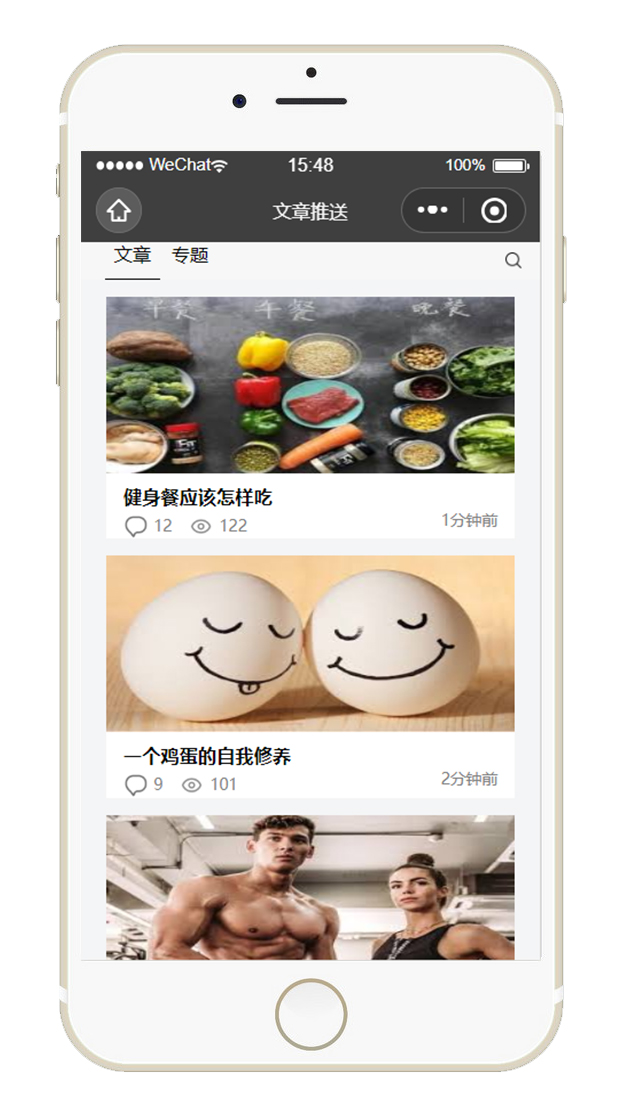
\includegraphics[width=11cm]{fig/!17}
	\end{figure}
	
	\newpage
	
	\item\textbf{饮食圈}
	
	这个模块推送各个用户发表的自己的饮食计划以及体验感受,我们提供了评论、收藏和点赞功能,在评论区用户可以根据感兴趣的话题进行交流。模块会根据动态发布时间和点赞收藏数来优先推送最新和精选动态。我们采用用户动态共享的方式,营造关系融洽,积极向上的社区氛围,进而吸引更多用户的眼球,促使用户对健身饮食以及本程序进一步的了解。
	
	\begin{figure}[!htb]
		\centering
		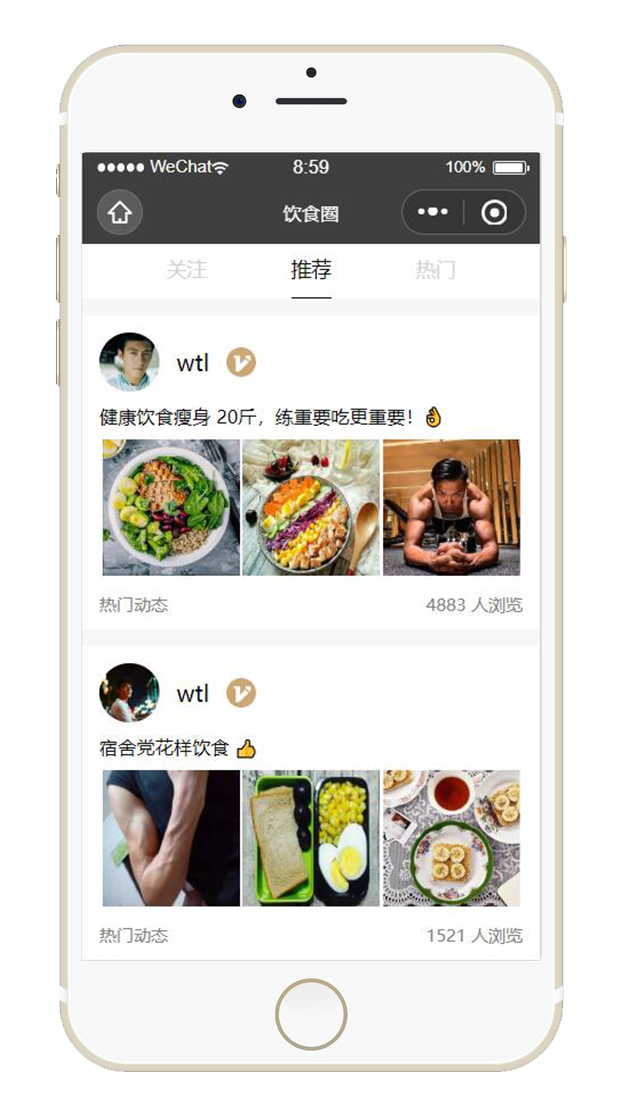
\includegraphics[width=8.5cm]{fig/!4}
	\end{figure}
	
	\newpage
	
	\item\textbf{一键选购食谱}
	
	“食刻Diet”为每一位用户提供多样化的食谱以供选择,如果对于用户选择好的食谱,我们提供所有原料配送,让客户能做不出户就享受到最新鲜的食材和最优质的服务。
	
	我们的平台为VIP用户提供了制作食谱的功能。用户可以听取营养师的建议,执行私人营养师给定的食谱,但是,在有些情况下,用户可能会对食谱中的一些食物过敏、厌恶或是价格等原因无法食用,这时候用户可以通过平台提供的制作食谱功能,自定义自己想要的食谱,对无法采购到或其他原因无法食用的食物进行等热量替换。
	
	用户还可以为自己限定每日热量摄入上限,在食谱中选择每天计划食用的食物及其重量,并对所选食物进行热量统计。如此,用户便可以通过将限定热量与已选食物热量进行对比,从而及时调整自己食谱。
	
	\newpage
	
	\begin{figure}[!htb]
		\centering
		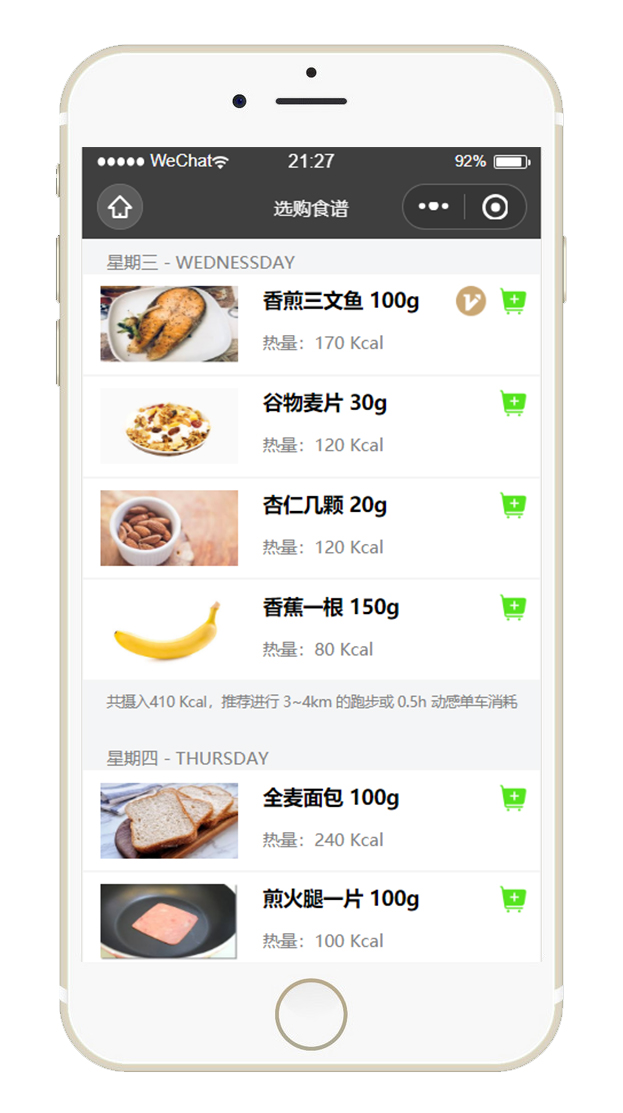
\includegraphics[width=10cm]{fig/!13}
	\end{figure}
	
	\newpage
	
	
	
	\item\textbf{我的菜篮子}
	
	我的菜篮子中显示出用户已购买的食材详情,用户还可以根据个人需求对各类食材进行单独选购或者在已有食材基础上增加购买量。
	
	\begin{figure}[!htb]
		\centering
		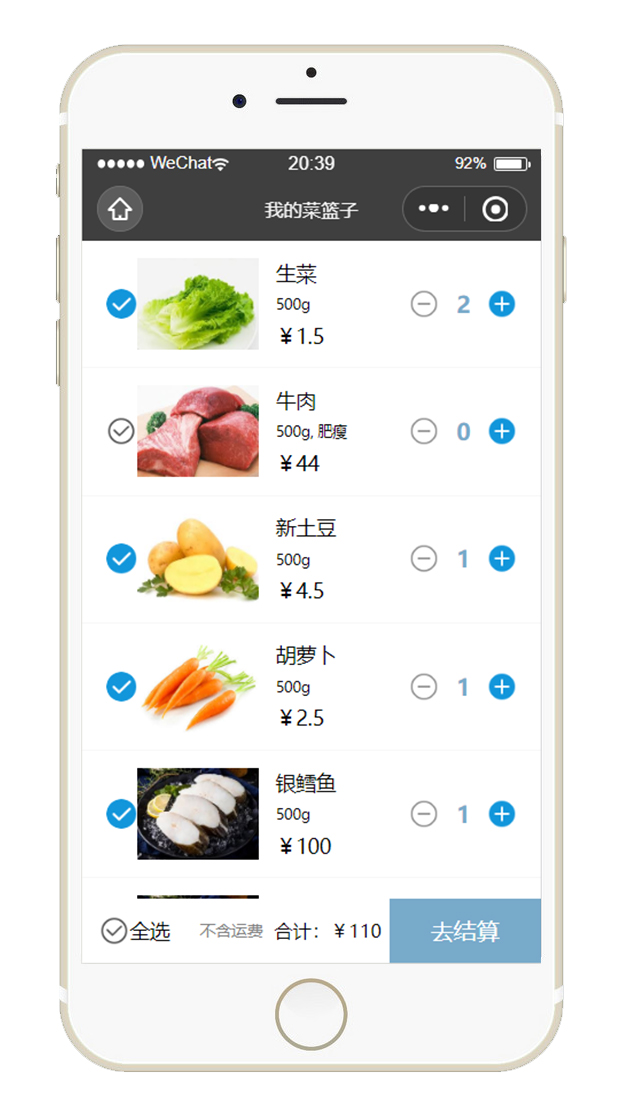
\includegraphics[width=10cm]{fig/!3}
	\end{figure}
	
	\newpage
	
	\item\textbf{查看食物热量}
	
	在这个模块中,用户可以查询所有食物的热量,及其热量计算公式,如红薯xx卡路里/kg,进而能够精确计算出自己一天摄入的热量,并自己进行控制,从而能够更好的控制自己的身材。
	
	
	
	\item\textbf{我的饮食计划}	
	\parpic{%
		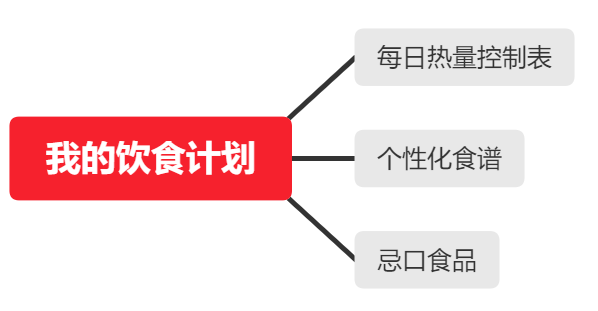
\includegraphics[width=7cm]{fig/40}}
	
	我们根据用户在“我的身体状况”中填写的身体各项指标,系统能够智能地为用户推荐一系列的饮食计划、食谱等,设定每日热量控制表,表明忌口食品,培养用户良好的健康饮食习惯,以实现用户的个性化健身目标。	
	
	\item\textbf{我的配送}
	
	配送功能是本平台核心功能之一。我们会根据完成的食谱进行每周的食材采购,以帮助用户更加方便地进行自己的饮食计划而不会因为食材采购问题的问题再次放弃。在配送的食材包中也附有打印好的食谱卡片。食谱的内容包括:对菜品的简要描述、食用方式、特殊说明(是否含坚果和麸质)、食材和配料用量、营养含量以及图文步骤。
	
	我们和超市进行合作,我们平台的最终目的是作为一个与连锁超市进行合作的电商平台,我们生成的原材料采购建议可以直接与超市进行对接,采购建议可以直接生成订单在超市内进行打包,帮助用户省去进入超市挨个挑选称重的麻烦,而可以直接在超市自提打包好的原材料八国或是采用配送外卖的形式在最近的超市下单后根据填写的“我的地址”配送到家。
	
	用户可以自行选择配送日期和地点,并可以在距离下次配送5天以前随时修改、暂停或取消订购。
	
	
	
	\item\textbf{我的饮食记录}		
	\parpic{%
		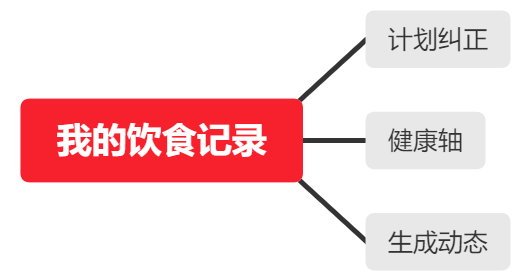
\includegraphics[width=7.5cm]{fig/41}}
	
	健康饮食计划平台能够为用户统计每周三餐情况以及展示计划完成情况,系统能够为用户提供最近一周的饮食数据,还会根据饮食情况给出健康的建议,以帮助用户的生活更健康。
	
	我们还建立了健康轴,健康轴能够根据用户的饮食记录与健康计划情况进行成长,反应出用户的健康状况,并及时提供健康提醒。
	
	我们在此页面也可以直接生成饮食动态,与社区中的朋友进行交流分享经验和感受,这有助于我们形成更好的健身氛围。
	
	
	\item\textbf{我的身体状况}	
	
	每个人的身体状况都是不同的,身体状况包括身高、体重、体脂率,这是最基本的情况,更详细的身体状况可以通过健身房的体脂秤得到,例如身体各个部位骨骼肌含量等,我们根据每个人不同的身体状况以及每个人对自己的预期状况进行计划的制定
	
\end{itemize}

\newpage
%%
\subsubsection{三级页面架构}

\begin{itemize}
	\item\textbf{食材特点}
	
	既根据中医养生理念给出食物习性即:寒、凉、温、热等不同的“四性”,也有世界卫生组织给出的食品热量等相关标准,让用户对所食之物有更多了解。
	
	\item\textbf{热门话题推送}
	
	每周定期总结当前一周内健康饮食领域内的新鲜事,根据时令推送当前季节的新鲜佳肴美味。根据用户的喜好推送美食达人的饮食日志等。
	
	\item\textbf{搜索记录}
	
	根据用户输入的关键词进行匹配,显示出符合程度较高的官方文章、动态或其他用户,以供当前用户直接进行查询。
	
	
	\item\textbf{智能推荐}
	
	许多健身初学者在起初健身时,最大的一个难点之一就是不知道如何进行饮食控制。健身圈子里面常说“三分练七分吃”,可见在健身方面,饮食所占的比重不亚于锻炼,吃什么,怎么吃,吃多少已经成为了许多健身初学者的难题。这时候,他们十分需要一个私人营养师可以根据自己的个人情况给自己推荐合适的健身餐。只有饮食和训练同时进行,我们健身才会有效,从而实现健身目标。
	
	食刻 Diet平台根据用户的历史信息选择性为用户推送适合他们的健康饮食食谱。	
	
	\newpage
	
	\item\textbf{私人营养师推荐}
	
	在充值VIP后,用户可以与营养师进行交流,询问健身餐相关的问题,并且营养师会根据用户的身体情况和预定目标提供一份合理的饮食表,并实时对VIP用户的个人饮食记录进行查看,以人为纠正用户在饮食上出现的问题。
	
	\item\textbf{查看运动员饮食}
	
	对于有些用户,似乎基本的增肌和减脂餐不能完全满足用户需求。例如一个热爱篮球的非专业运动员,他要做的可能不仅仅是单纯的增肌和减脂,他更需要一些提高弹跳力和耐力的训练,但这些训练往往要搭配专门类型的食材。因此,VIP用户除了查看最基本的减脂餐和增肌餐,还可以查看运动员食谱,在职业运动员一日三餐的基础上进行一些改变,从而制定一份适合自己的食谱。
	
	\item\textbf{发布饮食记录}
	
	用户可以把自己每日饮食状况分享到饮食圈中,让更多人看到自己的健康饮食情况,从而对用户的坚持健康饮食形成正向反馈。
	
	\newpage
	
	\begin{figure}[!htb]
		\centering
		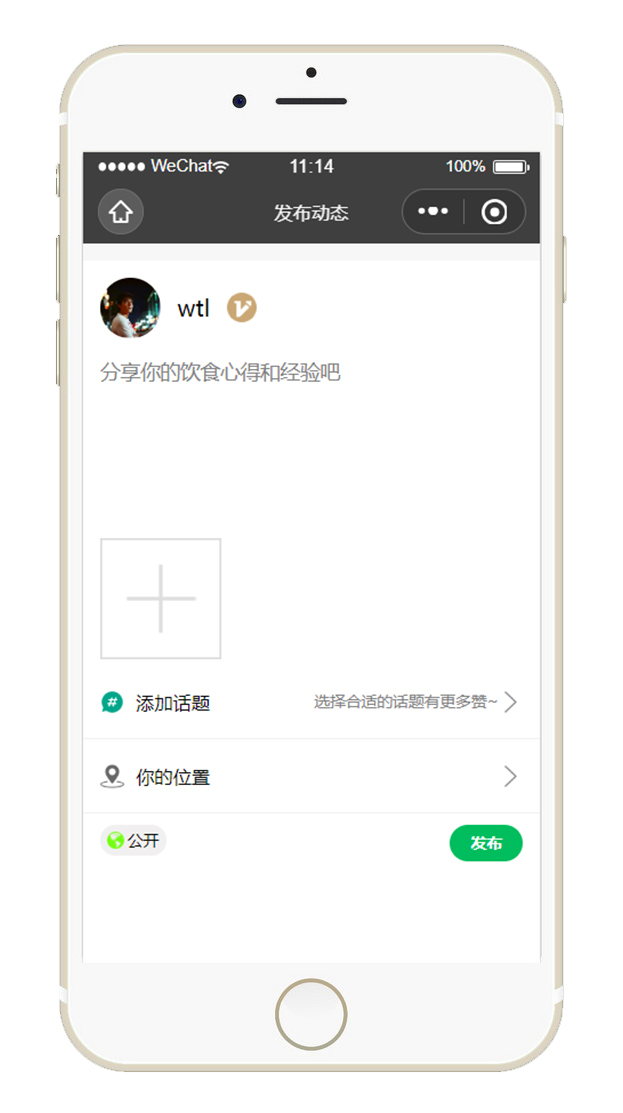
\includegraphics[width=11cm]{fig/!5}
	\end{figure}
	
	
\end{itemize}


%-----------%
\subsection{商家界面}




\subsubsection{页面架构}

\begin{itemize}
	
	\item 首页
	
	\begin{figure}[!htb]
		\centering
		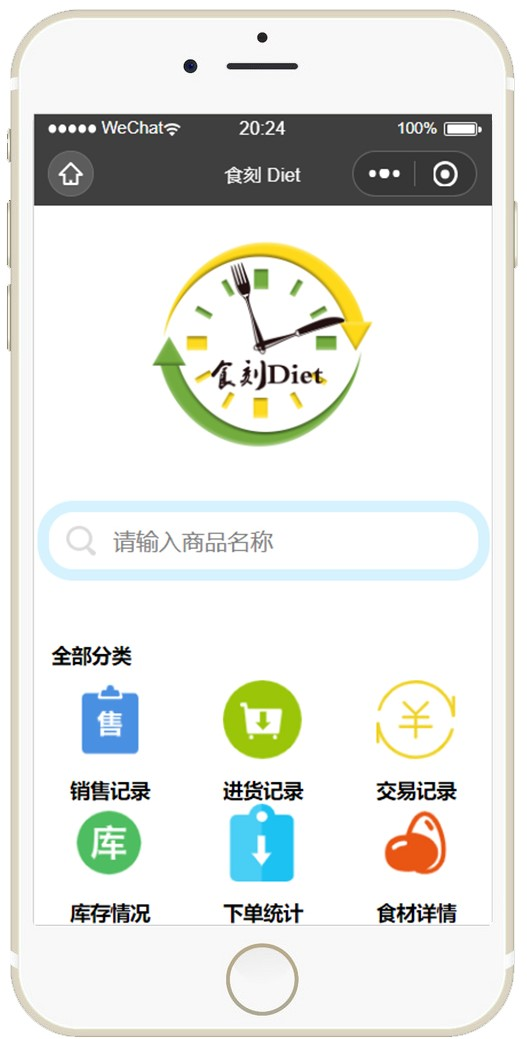
\includegraphics[width=9cm]{fig/!10}
	\end{figure}
	
	\item 库存信息同步
	
	对于供货商端,利用库存信息同步的功能可以帮助平台迅速掌握订单的安排问题,既能减少骑手在到达供货商而无法取到食材浪费的时间,又能提供配送效率,给用户更好的消费体验。
	
	在库存信息同步界面,供货商有更新商品库存量和交易日期的权限,同时,供应商端能通过库存查询到最新订单信息和商品剩余量,有利于供应商更好地调节供给。
	
	\newpage
	
	\begin{figure}[!htb]
		\centering
		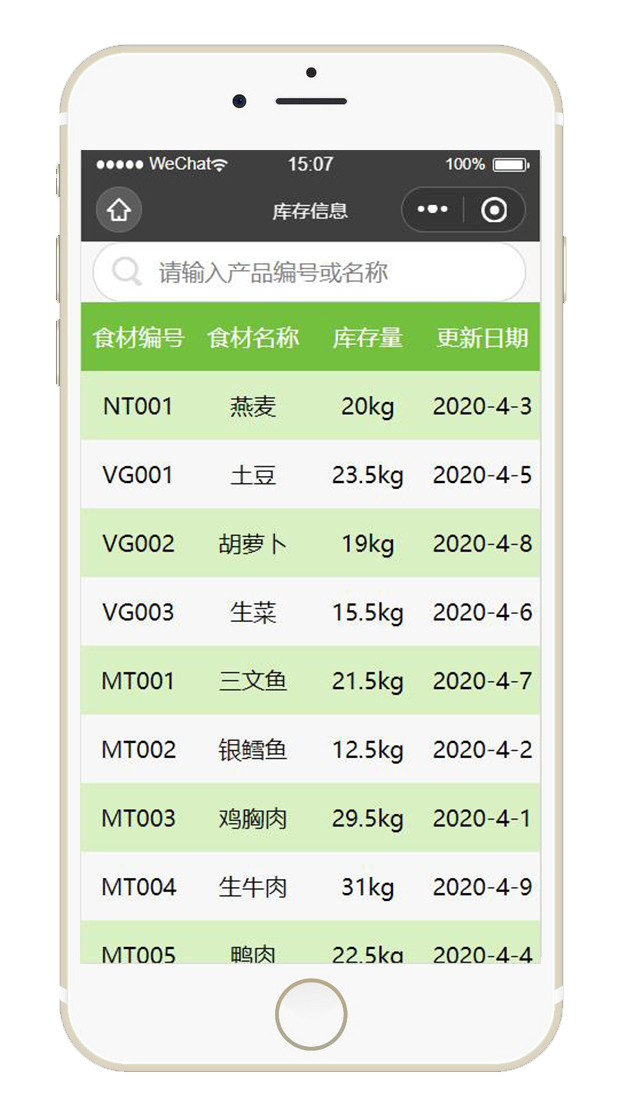
\includegraphics[width=11cm]{fig/!11}
	\end{figure}	
	
	\newpage
	
	\item 订单处理
	
	商家在订单处理界面能够对用户的订单进行确认和拒绝,
	\begin{figure}[!htb]
		\centering
		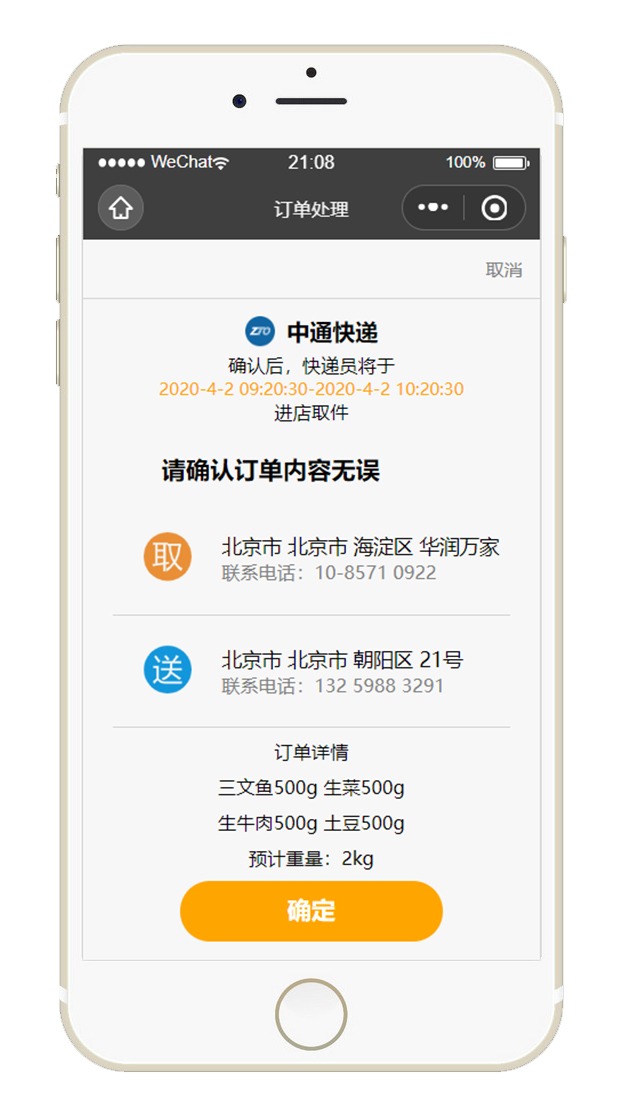
\includegraphics[width=10cm]{fig/!7}
	\end{figure}
	
\end{itemize}


%-----------%
\subsection{骑手界面}

\subsubsection{页面架构}

\begin{itemize}
	\item 订单信息
	
	骑手没有查看用户订单内容的权限,这是为了保证用户的隐私。骑手页面的订单信息仅限于卖家买家地址、货物件数以及联系卖家买家的联系界面。
	
	\newpage	
	
	\begin{figure}[!htb]
		\centering
		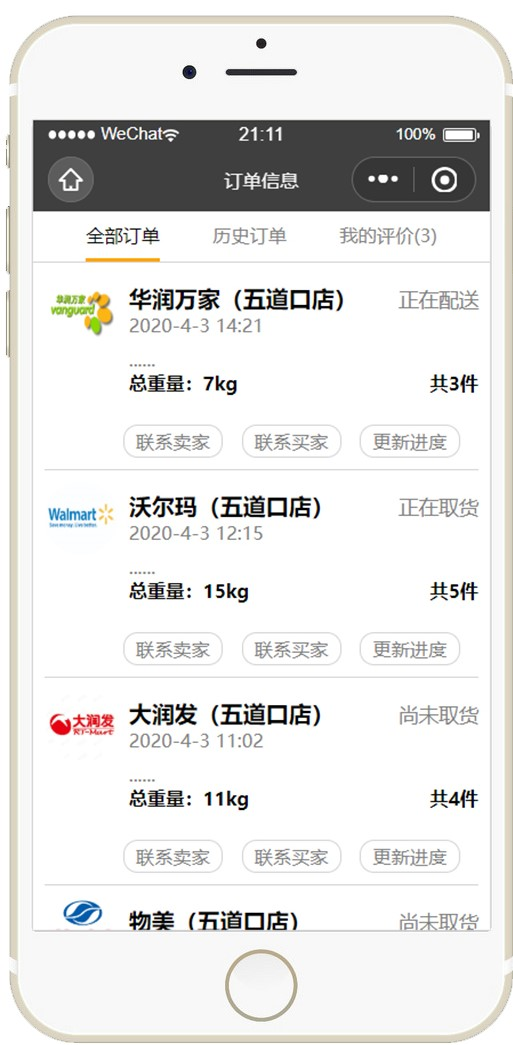
\includegraphics[width=10cm]{fig/!8}
	\end{figure}
	
	\newpage
	
	\item 派送位置同步
	
	骑手根据配送进度进行实时更新,以便用户合理掌握配送预计时间,给用户带来更便捷的使用体验。
	
	\begin{figure}[!htb]
		\centering
		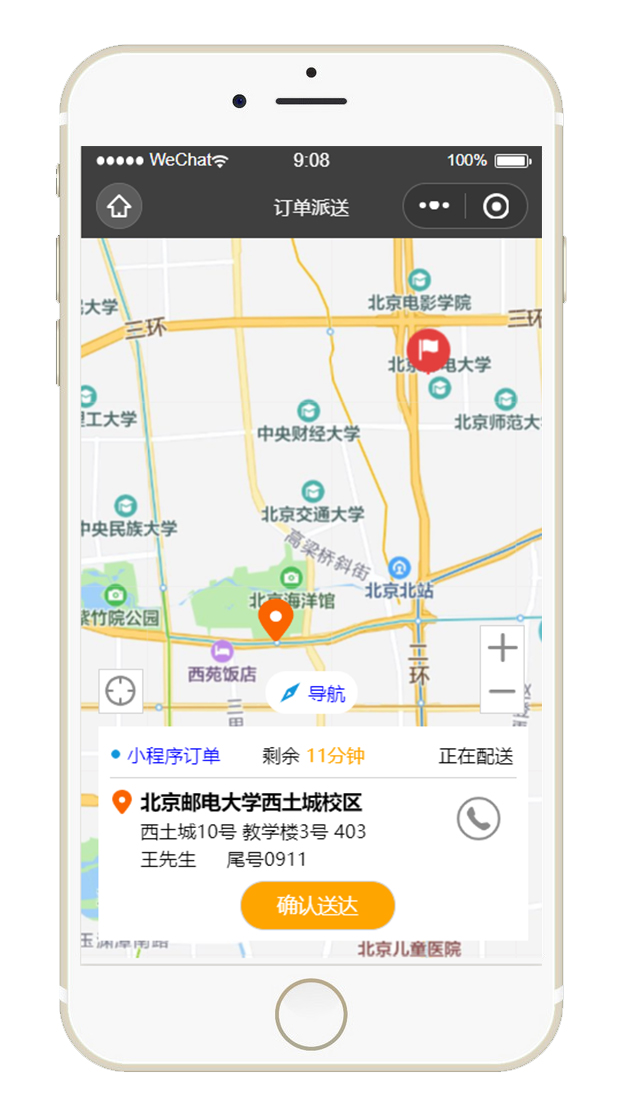
\includegraphics[width=10cm]{fig/!12}
	\end{figure}
	
	\newpage
	
	\item 接单中心
	
	接单中心显示了配送本订单的收入,有订单配送预计时间、订单取送位置等信息。骑手在这个界面进行抢单,确认配送的订单将会在订单信息页面中显示。	
	\begin{figure}[!htb]
		\centering
		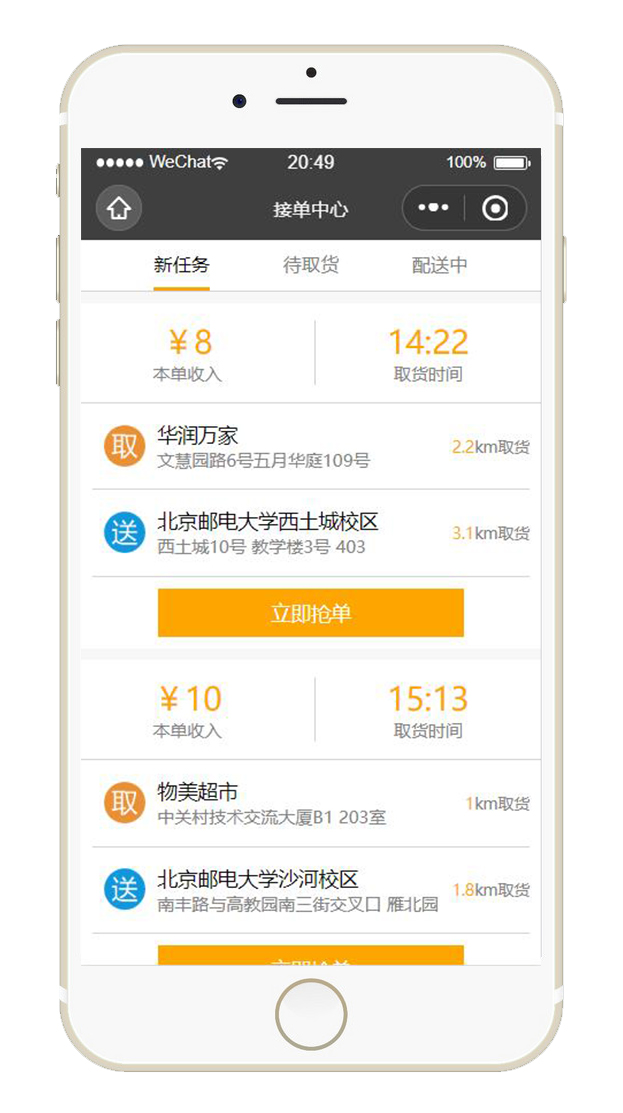
\includegraphics[width=10cm]{fig/!9}
	\end{figure}
	
	
\end{itemize}

%---------------------------------------------------------------------------------------------%
%---------------------------------------------------------------------------------------------%
\section{公司战略}
%-------------------%
\subsection{公司简介}
食客团队是由管理科学与工程、电子商务、计算机、电子专业的五名本科生组成。我们团队本着“健康生活,健康饮食”的理念,希望打造出一个集饮食私人化定制与配送为一体的一站式的食品销售平台。同时,通过食刻 Diet的饮食分享等新颖功能,我们希望能让更多的人关注饮食健康,为大众提供更加方便快捷的健康饮食体验。
\begin{figure}[!htb]
	\centering
	
\includegraphics[width=8cm]{fig/logo}
	\caption{食客团队Logo}
\end{figure}
%------------------%	
\subsection{文化理念——健康,贴心,创新}
公司在致力于搭建健康饮食平台的同时,注重健康饮食理念,在配送菜品的选取上,我们力争“三最”:最新鲜的食材,最健康的做法,最真实的味道。在最短的时间,把最新鲜的食材送到用户手中,给用户提供最健康的菜谱供用户选择,让用户足不出户就能体验到舌尖上的健康美味。

公司注重用户体验,用心为用户考虑。针对健身用户,我们提供食物热量配算;针对有小朋友的用户,我们提供多种儿童成长健康套餐;针对中老年用户,我们提供低脂低盐低胆固醇的健康菜谱。注重换位思考,公司定期组织市场调研,学习最新饮食理念,努力为用户提供一流的饮食体验。

公司注重创新精神的培养,鼓励团队开发新的餐饮菜谱,管理者以营造一个和谐、有活力、敢创新的公司氛围为目的,培养饮食研发团队的创新意识。公司采用定期邀请营养学专家、餐饮界名厨开展讲座等方式,激发团队创新活力,让用户享受健康饮食新体验。

%-------------------%	
\subsection{发展规划}
\subsubsection{短期规划}
公司的短期规划主要集中在:小程序上线并实现健康饮食定制、配送指定菜谱食材、各类菜谱食材热量计算等基本功能;通过多种宣传方式扩大品牌知名度实现用户推广;让健身人群和各类对健康饮食有不同需求的人群了解食刻 Diet小程序,增加用户量,提高公司知名度。短期规划具体内容如下:
\begin{enumerate}
	\item[(1)]
	
	\setlength{\parindent}{2em}完成小程序架构,实现小程序上线运营,逐步实现饮食选择,原料配送,计算饮食热量等功能。
	
	\item[(2)] 
	
	\setlength{\parindent}{2em}利用抖音、微博、知乎等新媒体平台和Keep、Fit等运动健身平台宣传食刻 Diet的健康饮食理念,提高食刻 Diet知名度。
	
	\item[(3)] 
	
	\setlength{\parindent}{2em}首先在北京、上海、深圳等一线大都市开启配送服务,利用都市庞大的客户群体,更好的服务那些希望健康饮食,但是由于各种时间原因而不得的客户。
	
	\item[(4)]
	
	\setlength{\parindent}{2em}在合适的时间推出优惠政策和促销活动,如免费配送,菜品优惠等,迅速扩张都市群体的用户数量。
\end{enumerate}

这一短期规划的实现预期需要1年时间。

\subsubsection{中期规划}
公司的中期规划主要致力于提供饮食分享评论功能;推送各类食材介绍、健身明星饮食表以及更多热门话题推荐;提供根据历史饮食喜好的动态日常更新;针对VIP用户的更多可选择健康饮食菜谱;原料采集产地化;配送订单实时更新等进一步服务。

\begin{enumerate}
	\item[(1)]进一步完善功能区布局,在首页推送各类食材知识、明星健身餐等热门话题,让用户了解当下健康饮食理念。
	
	\item[(2)] 推出饮食分享活动,设置“一键分享”的功能,链接国内常用社交网站或软件(如:微博、抖音、微信朋友圈等等)。这一方面可以进一步扩大公司影响力;另一方面,让用户享受到健康饮食带来的互动,对健康饮食起到正向促进作用。
	
	\item[(3)] 扩大公司服务的地域范围,业务覆盖全部一线城市和少数经济发达的二线城市。
	
	\item[(4)]鉴于当前公司已经积累了一部分用户群体,适时开展会员VIP专享的私人饮食定制,提供VIP专属服务。
	
\end{enumerate}

中期规划的实现需要2-3年时间。

\subsubsection{长期规划}
公司的长期规划是让食刻 Diet健康饮食的理念深入更多人的心中,让每一个家庭都能享受到食刻 Diet提供的饮食配送服务。希望公司形象成为健康饮食的代名词,食刻 Diet能够成为健康饮食的象征。

\begin{enumerate}
	\item[(1)]采用公关营销与情感营销相结合的营销方式,分步、分层次实施,最终与各种社会力量建立良好的关系,使企业有一个良好的生长环境从而实现产品品牌价值的积累。
	
	\item[(2)]加强公司内部管理营销,制定人才战略和创新战略,不断保持公司创造力,尽全力满足用户要求,为用户提供一流的服务体验。
	
	\item[(3)] 坚持培养“健康,贴心,创新”的企业文化,关注食品健康、饮食安全问题,把推动社会形成健康饮食的文化潮流作为公司的社会责任。
	
	\item[(4)]关注每一位员工的职业体验,完善各项福利,提高员工的工作积极性和企业忠诚度。
	
\end{enumerate}	

长期规划的实现需要4年时间。
%-------------------%

\newpage

\subsection{发展策略}

公司为达到长期稳定发展,制定了以下基本发展策略,如图\ref{fazhan}:

\begin{figure}[!htb]
	\centering
	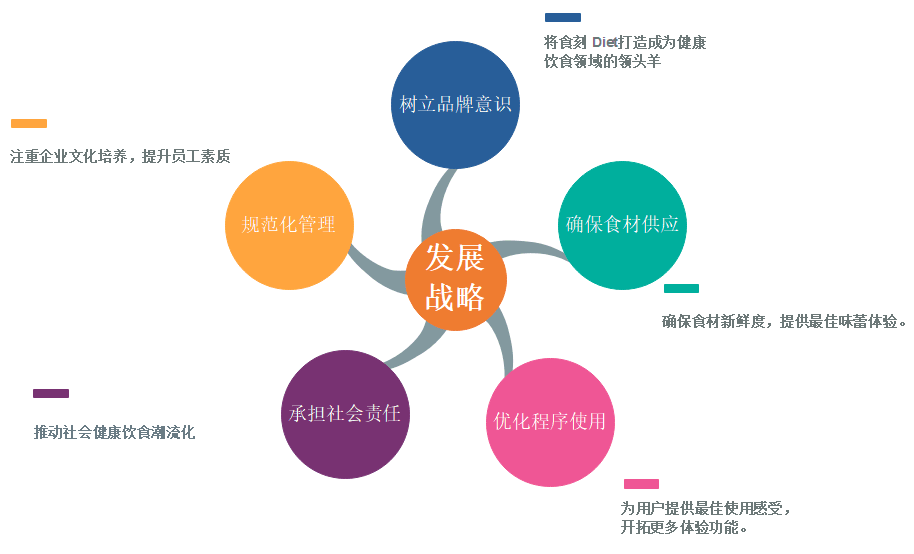
\includegraphics[width=12cm]{fig/9}
	\caption{食刻 Diet发展策略}\label{fazhan}
\end{figure}


\begin{enumerate}
	\item[(1)]确保供应食材的安全性、新鲜度,为用户提供最佳味觉体验。
	
	\item[(2)]不断优化小程序使用细节,开拓更多服务模块。
	
	\item[(3)]树立品牌意识,将食刻 Diet打造成健康饮食领域的领头企业。
	
	\item[(4)]对公司内部员工进行规范化管理,注重企业文化培训。
	
	\item[(5)]把营造社会健康饮食风气作为企业的社会责任,推动健康饮食的潮流。
	
\end{enumerate}	

%---------------------------------------------------------------------------------------------%
\section{商业模式}

\begin{figure}[H]
	\centering
	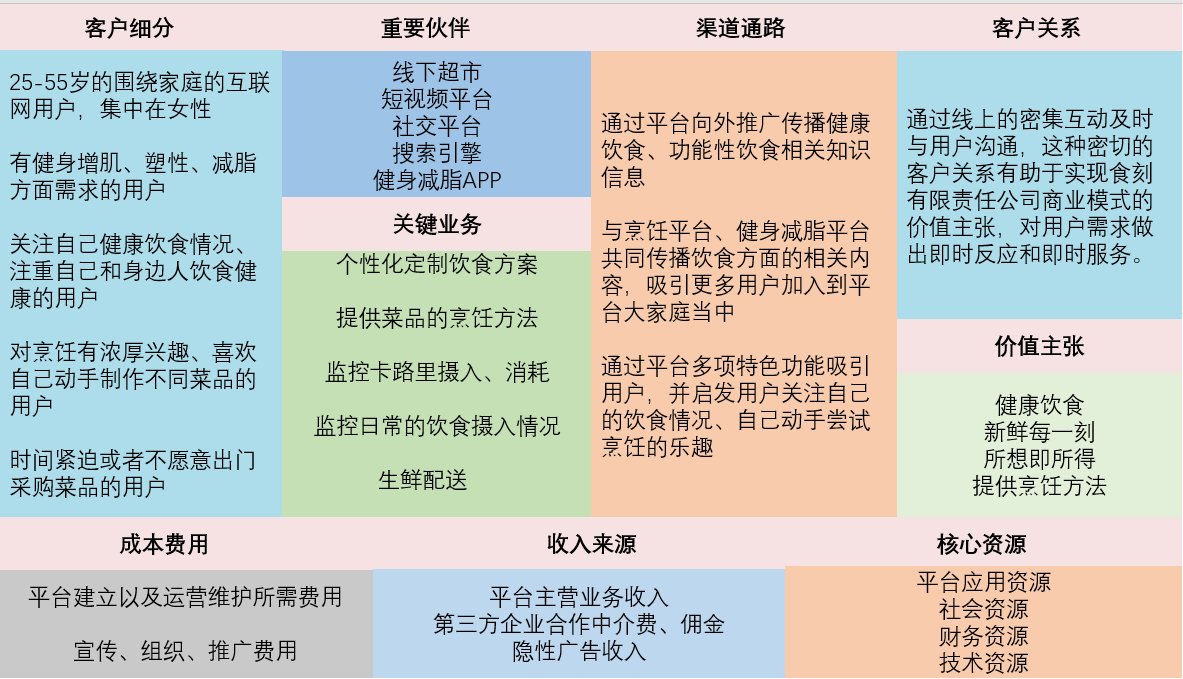
\includegraphics[width=13cm]{fig/shangyehuabu}
	\caption{商业画布}
\end{figure}
%--------------%
\subsection{重要伙伴}

\subsubsection{线下超市}

\begin{figure}[!htb]
	\centering
	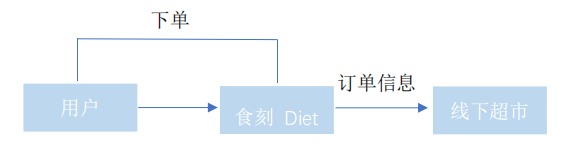
\includegraphics[width=12cm]{fig/yonghu-chaoshi}
	\caption{线下超市-平台 \ 关系}
\end{figure}

食刻有限责任公司以建立网络式的饮食攻略平台为核心,为用户与线下各大超市搭建中间桥梁。“食刻Diet”小程序在平台内专设生鲜采购模块,平台自动生成的菜品原材料采购建议可以直接与线下超市进行对接,采购建议可以在平台上直接生成订单在超市内部进行选购、称重、打包、配送,为用户提供新鲜的食材和灵活的订购方式,改变消费者食品采购方式。平台为合作超市带来商业价值的同时,也能实现本公司自身的盈利。


\subsubsection{短视频平台}

以目前较火的短视频行业为切入点,通过制作一些精美引流的烹饪短视频在抖音、快手、火山小视频等短视频应用上定期常态化投放。在制作视频的同时将食刻有限责任公司旗下主推产品“食刻Diet”小程序特点、平台内容积极融入进去,获得新媒体平台的支持,为“食刻Diet”做相关的推广,遵循平台的相关政策,争取其对本公司有关活动的推广与宣传。

\subsubsection{社交平台}

利用微信、微博、小红书等新媒体社交平台,引导大家关注健康饮食、功能性饮食推广并我们的品牌。利用微博博主、 微信公众号推送、小红书博主等进一步推广“食刻Diet”小程序。

\subsubsection{健身减脂APP}

食刻有限责任公司将积极与keep、fit等影响力较高的健身减脂APP进行交流合作,通过价格竞标购买其广告版面,宣传营销;通过互置链接,互推产品等方式,共享客户群,扩大用户数额,达到互利共赢。

\subsubsection{搜索引擎}

公司会在百度、google等网站进行搜索推广。 本公司将主要采取竞价搜索的方式,对:健康饮食、减脂、健身、烹饪、 美食等关键词进行搜索排名提高,以此来提升“食刻Diet”小程序的访问量,提高公司的知名度。

%--------------%
\subsection{价值主张}

食刻有限责任公司从广大用户群体的饮食需求出发,打造一个科学、便捷、私人定制的饮食服务平台。针对用户的个人偏好、健康饮食、功能性饮食等需求,为用户定制个性化饮食搭配。坚持培养“健康,贴心,创新”的企业文化,关注健康饮食、饮食安全问题,把推动社会形成健康饮食的文化潮流作为公司的社会责任。

\begin{itemize}
	\item 健康饮食
	
	根据用户的口味个人、功能饮食、摄入卡路里限制等需求,平台结合营养学计算公式,对应推荐健康多样化的菜谱、饮食安排表
	
	\item 新鲜每一刻
	
	用户买到的和吃到的,都是新鲜的。今天买的今天吃,一顿刚刚好
	
	\item 所想即所得
	
	满足用户随时随地不同场景的需求;线上线下高度融合,提供全天候的便捷服务
	
	\item 提供生成烹饪方法
	
	细致化的菜谱将会提供原材料清单、制作方法、教学视频,为用户省去纠结吃什么、怎么做、采购食物材料等一系列复杂过程
	
	
\end{itemize}

%--------------%
\subsection{收入来源}

\begin{itemize}
	\item 平台主营业务收入
	
	会员充值、用户购买定制化套餐、用户在平台下单购买食材
	
	\item 第三方企业合作中介费、佣金
	
	线下超市、骑手配送、相关APP、新媒体平台等合作费用
	
	\item 隐性广告收入
	
	定期活动的冠名费、赞助费,介绍相关公司的报告内隐含的宣传费等 
	
\end{itemize}

%--------------%
\subsection{核心资源}
\subsubsection{平台应用资源}

由使用者的各项信息数据整合收集,为平台提供反馈协调所需的重要保障。

\subsubsection{社会资源}

多项第三方企业对接资源,包含相关APP、网站、超市等。在保证用户获得优质服务体验的基础上,平台也能够拥有更强的行业竞争力。

\subsubsection{财务资源}

“食刻Diet”作为食刻有限责任公司的主要项目,获得食刻有限责任公司的直接投资,拥有强大的资金优势。

\subsubsection{技术资源}

研发团队依靠先进的算法系统,提供一个拥有强大技术优势,从而支撑稳定的收入来源。

%--------------%
\subsection{成本费用}

\begin{itemize}
	\item 平台建立以及运营维护所需费用
	
	内容更新、信息管理、数据存储 
		
	\item 宣传、组织、推广费用
	
	需要借助人力资源达到高效运作
\end{itemize}
%--------------%
\subsection{关键业务}
\subsubsection{个性化定制饮食方案}

根据不同用户的身体状况、口味偏好、功能性饮食需求,“食刻Diet”会为其量身定制个性化合理的饮食方案。

\subsubsection{提供菜品的烹饪方法}

“食刻Diet”收集整合各种菜品的制作方法,配以图文说明、演示讲解视频,方便用户学习制作更多美味的菜肴。

\subsubsection{监控卡路里摄入、消耗}

“食刻Diet”平台提供卡路里监控页,有健身、减脂需求的用户可查看每天,或者一个时间段内的卡路里摄入情况,进行科学合理的健身、减脂。

\subsubsection{监控日常的饮食摄入情况}

平台提供饮食情况记录表,对一定时间内用户的碳水化合物、蛋白质等营养物质的摄入情况进行统计分析,监控用户的均衡膳食情况。在用户某方面物质摄入偏少或过多时进行温馨提醒。

\subsubsection{生鲜配送}

平台内有专设生鲜采购模块,菜谱内也直接附带购买链接,用户可自行在家挑选、下单,等待食材配送上门。

\subsubsection{按需订购}

平台积极响应国家号召,旨在方便用户落实“光盘行动”。平台提供“单人份”、“双人份”、“三人份”等不同规格的食材购买方案,用户可以根据实际用餐人数,在下单时自行选择,或直接输入用餐人数,争取做到一次购买量,一次食用,避免不必要的浪费的发生。

%--------------%
\subsection{客户关系}

“食刻Diet”通过线上的密集互动及时与用户沟通,这种密切的客户关系有助于实现食刻有限责任公司商业模式的价值主张,对用户需求做出即时反应和即时服务。

%--------------%
\subsection{渠道通路}

\begin{itemize}
	\item
	通过平台向外推广传播健康饮食、功能性饮食相关知识信息,让更多消费者关注平台
	
	\item 通过平台多项特色功能吸引用户,并启发用户关注自己的饮食情况、自己动手尝试烹饪的乐趣
	
	\item 
	与烹饪平台、健身减脂平台共同传播饮食方面的相关内容,吸引更多用户加入到平台大家庭当中,感受其带来的方便与快捷服务 
		
\end{itemize}

%--------------%
\subsection{客户细分}
\begin{itemize}
	\item 从用户属性角度看,“食刻Diet”的目标用户是 25-55岁的围绕家庭的互联网用户,集中在女性
	
	\item 有健身增肌、塑性、减脂方面需求的用户
	
	\item 关注自己健康饮食情况、注重自己和身边人饮食健康的用户
	
	\item 对烹饪有浓厚兴趣、喜欢自己动手制作不同菜品的用户
	
	\item 时间紧迫或者不愿意出门采购菜品的用户
		
\end{itemize}


%---------------------------------------------------------------------------------------------%
\newpage
%---------------------------------------------------------------------------------------------%		
\section{管理团队和运营组织}
%-------------------%	
\subsection{公司组织架构}
我们建立了一种决策权的划分体系以及各部门的分工协作体系。组织架构需要根据企业总目标,把企业管理要素配置在一定的方位上,确定其活动条件,规定其活动范围,从而形成了相对稳定的科学的管理体系。


\begin{figure}[!htb]
	\centering
	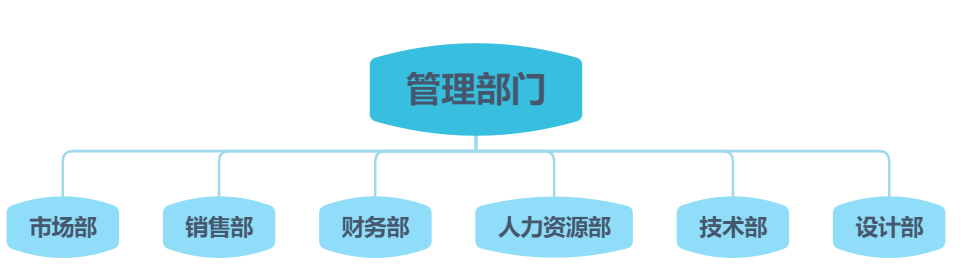
\includegraphics[width=12cm]{fig/10}
\end{figure}

\begin{figure}[!htb]
	\centering
	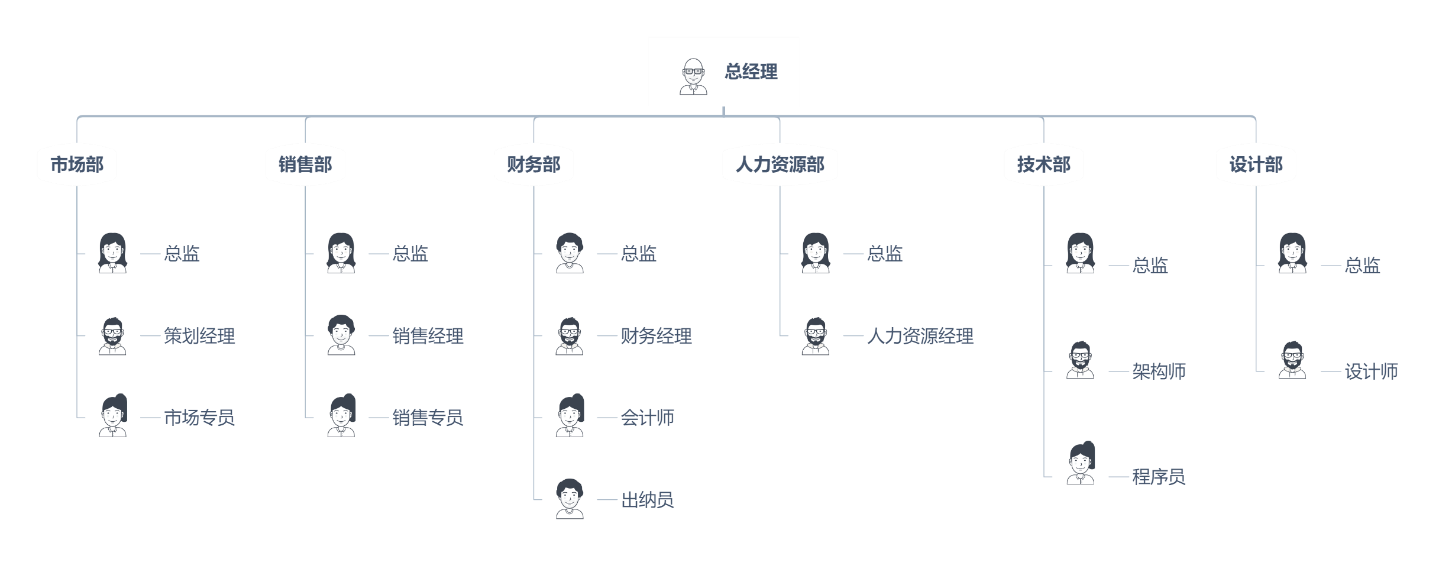
\includegraphics[width=14cm]{fig/11}
%	\caption{盈利模式}
\end{figure}

\newpage

\begin{itemize}
	
	\item \textbf{市场销售部}
	
	市场销售部需要制定年度营销目标计划,对健身人群的消费心理和行为的调查,对其他健身竞争平台的价格、促销手段等进行收集、整理和分析,做出销售预测,提出健身食材配送的未来市场的分析、发展方向和规划,进行食材配送和食谱定制的促销活动的策划及组织。

	\begin{figure}[!htb]
		\centering
		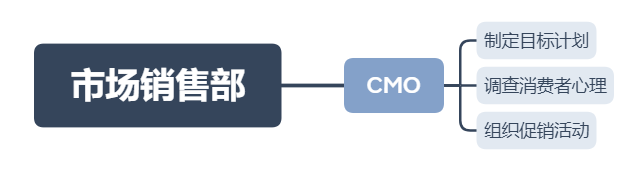
\includegraphics[width=10cm]{fig/12}
		%	\caption{盈利模式}
	\end{figure}
	
	 
	\item \textbf{财务部}
	
	财务部门的目标为:实现利益最大化,管理当局收益最大化,企业财富最大化以及社会责任最大化。财务部要起草公司年度经营计划,组织编制公司年度财务预算,执行、监督、检查、总结经营计划和预算的执行情况,并提出调整建议。
	\begin{figure}[!htb]
		\centering
		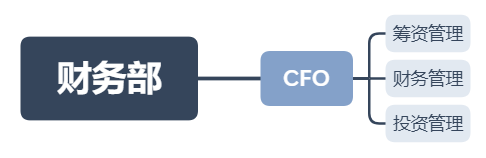
\includegraphics[width=9cm]{fig/13}
		%	\caption{盈利模式}
	\end{figure}

	\item \textbf{人力资源部}
	
	人力资源部需要选择最适合单位和岗位要求的人才,通过培训教育,不断提升员工的专业技能和综合素质,改善绩效,提升工作效率和员工价值,并且把符合岗位任职资格要求且具有完成岗位职责的能力与技能的员工,放在合适的职位上,并发挥出最大的潜能。
	\begin{figure}[!htb]
		\centering
		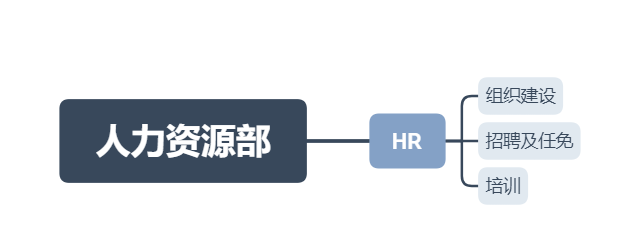
\includegraphics[width=10cm]{fig/14}
		%	\caption{盈利模式}
	\end{figure}
	
	
	\item \textbf{设计部}
	
	设计部主要负责健身平台的设计,根据产品调研研发本平台的各项业务服务,并进行创新,继续研发新的功能。根据平台留言板,了解用户需求,解决用户的困难,为用户提供更多的便捷。
	\begin{figure}[!htb]
		\centering
		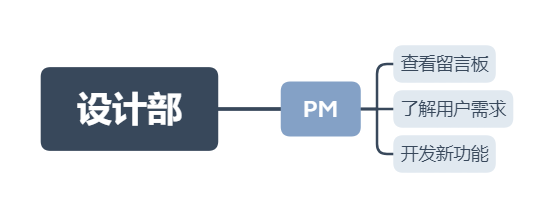
\includegraphics[width=10cm]{fig/15}
		%	\caption{盈利模式}
	\end{figure}
		
	
	\item \textbf{技术部}	
	技术部需要维护小程序的页面,健身社区中动态的维护,则需要维护数据库,并且根据设计部的需求进行技术上的实现,并对技术进行测试。
	\begin{figure}[!htb]
		\centering
		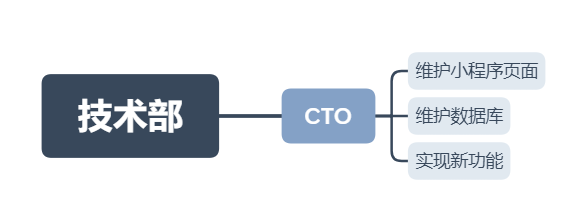
\includegraphics[width=10cm]{fig/16}
		%	\caption{盈利模式}
	\end{figure}
	
	
\end{itemize}


%-------------------%	
\subsection{公司组织管理}
\subsubsection{管理层}
\begin{figure}[!htb]
	\centering
	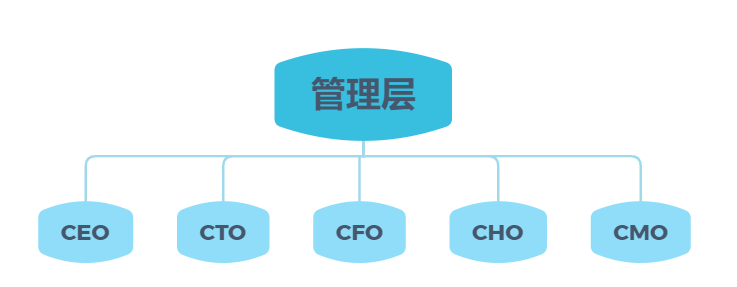
\includegraphics[width=10cm]{fig/17}
	\caption{管理层架构}
\end{figure}

\textbf{首席执行官 CEO——Chief Executive Officer}

首席执行官是在一个企业中负责日常事务的最高行政官员,主司企业行政事务,又称作总经理或最高执行长。
权责:
\begin{enumerate}
	\item 决策公司所有重大经营事项;
	
	\item 作为董事会的一员,参与并落实董事会的决策;
	
	\item 主持公司的日常业务活动;
	
	\item 经董事会授权,对外签订合同或处理业务;
	
	\item 高层管理团队的任免权;
	
	\item 调度资金分配,负责项目的投融资;
	
	\item 其他权责。
	
\end{enumerate}


\textbf{首席技术官 CTO——Chief Technology Officer}

首席技术官是技术资源的行政管理者。本公司属于网络公司,因此基于小程序的健身平台需要强大的技术支持。肩负重任的 CTO 职责如下:
权责:

\begin{enumerate}
	\item 制订有关技术的愿景和战略;
	
	\item 把握总体技术方向;
	
	\item 监督技术研究与发展(R\&D)的活动;
	
	\item 对技术选型和具体技术问题进行指导和把关;
	
	\item 完成所赋予的各项技术任务/项目;
	
	\item 其他权责。
	
\end{enumerate}

\textbf{首席财务官 CFO——Chief Financial Officer}

CFO也是公司与投资人沟通的一个“传声筒”。 公司的财务部门、会计部门、信息服务部门都归CFO管理。除了负责公司与投资人的公共关系,CFO要保证公司在发展过程中拥有足够的现金,要保证有足够的办公和生产经营空间。
权责:

\begin{enumerate}
	\item 审核集团公司的重要财务报表和报告;
	
	\item 参与审定公司的财务管理规定及其他经济管理制度;
	
	\item 对董事会批准的集团公司重大经营计划、方案的执行情况进行监督;
	
	\item 参与审定集团公司重大财务决策;
	
	\item 其他权责。
	
\end{enumerate}

\textbf{首席人力资源官 CHO——Chief Human Resource Officer}

\begin{enumerate}
	\item 制定公司人力资源的战略规划,督促公司人力资源战略的执行;
	
	\item 负责建立有效的沟通渠道和激励机制;
	 
	\item 全面集团化经营公司的负责人力资源部门的工作;
	
	\item 内部组织管理;
	
	\item 其他权责。
		
\end{enumerate}

\textbf{市场总监 CMO——Chief Market Officer}

市场总监是负责市场运营工作的高级管理人员,又称作市场部经理、营销总监。
权责:

\begin{enumerate}
	\item 寻找市场机会,确定市场营销战略和贯彻战略决策的行动计划;
	
	\item 在企业中进行营销思想的定位、指导和贯彻的工作;
	
	\item 负责企业市场营销战略计划的执行;
	
	\item 对企业市场行为进行监督;
	
	\item 负责或参与进行企业文化的建设;
	
	\item 其他权责。
	
\end{enumerate}

%---------------------%
\subsection{计划和总结}
“食刻 Diet“网络科技有限公司的规模会随发展规划的逐步扩张。管理层包括首席执行官(CEO)、首席技术官(CTO)、首席运营官(COO)、首席财务官(CFO)、市场总监(CMO)6名高层,以及技术部、产品部、销售部、市场部、财务部、人力资源部、行政部、客户服务部等8名部门负责人。


%---------------------------------------------------------------------------------------------%


\newpage	
\section{营销策略}

\subsection{营销概述}

随着经济社会的快速发展,经济的进步带给了人们在物质上的富强满足。然而,现在的亚健康已经围绕在我们的身边,几乎每一个人的身上都存在亚健康。对于工作繁忙、终日以快餐为食的都市工作者来说,居家烹饪已然成为一种挑战。要想在家做好一顿饭,需要研究食谱、去超市或菜场挑选所需食材,然后回来清洗、切配、腌制,最后开火加工,完成一顿饭的烹饪着实需要花费一番功夫。更不用说,其实对于很多人来说,做饭是一门讲究技术的手艺,根本不知从何下手。因此,居家烹饪成了很多互联网企业试图发力的地方,催生出大量的模式创新,如各种菜谱APP、美食视频网站等。

无论是菜谱类APP还是美食类视频网站,都是想让“下厨房”这件事变得更简单。但是,买菜、准备的过程还是费时费力。各类的美食公众号、健身公众号等自媒体也都有相应的板块与知识分享。但是由于这类板块只是他们内容的一部分或仅偶尔通过文章的形式进行分享,用户很难系统、方便的获取相关的饮食安排知识。

一方面,本公司旗下产品“食刻Diet”小程序采用一种全新的半成品生鲜电商C2B模式——提供设计好的食谱,并自动计算出累计后各种食材的需求量,用户可以一键下单,不需要一样一样食材去点击购买,用户只需在家中按步骤简单加工一下即可享用,而不会因为食材采购的问题再次放弃。

另一方面,为了培养更加健康的饮食习惯,“食刻Diet”小程序开发对用户的日常的餐饮习惯进行记录,对用户饮食摄取情况进行监控。提供饮食情况记录表,对一定时间内用户的碳水化合物、蛋白质等营养物质的摄入情况进行统计分析,监控用户的均衡膳食情况,并在用户某方面物质摄入偏少或过多时进行温馨提醒。平台通过板块的划分让用户可以个性化,并且通过与营养学家和厨师团队的合作,提供从食谱研制到食材供应的全套居家烹饪解决方案,从而为用户安排每餐热量的分配以及菜谱建议,用户也可以根据自己的喜好再每餐的推荐安排上进行合理的切换(例如一餐安排四百大卡的热量,我们以滑动菜单的形式来让用户自行自定义的选择在完成安排)。并且对用户的饮食内容进行分析,评估用户摄入内容对健康的影响,为用户普及饮食知识。特别是对于处于健身、减肥阶段的用户,“食刻Diet”小程序能够帮助用户制定合理的饮食计划:平台还提供卡路里监控页,用户可以查看每天,或者一个时间段内的卡路里摄入情况,进行科学合理的健身、减脂,健康减肥或是增肌。对于糖尿病患者、孕妇等特殊人群,“食刻Diet”可以为他们定制饮食方案,进行膳食结构监控。

\begin{figure}[!htb]
	\centering
	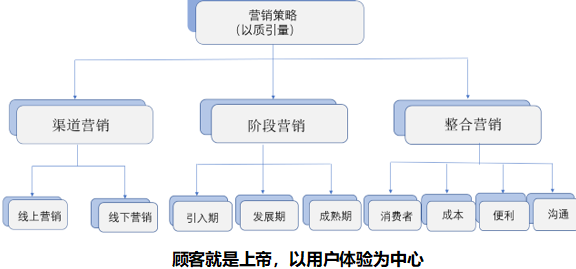
\includegraphics[width=14cm]{fig/21}
	\caption{营销方案图}\label{xsh}
\end{figure}

我们采取“一中心,两渠道,三阶段,四整合”的营销策略(如图\ref{xsh}),拓宽渠道、广泛合作、整合资源、精准营销,以认真的态度和专业的知识为用户提供高品质的服务,维护良好用户关系,培养用户习惯。 

 一中心:顾客就是上帝,以顾客为中心,以顾客的需求为导向,以质引量。

 二渠道:线上线下相互结合,协同发展。 

 三阶段:划分“引入期”“发展期”“成熟期”三个阶段。明确定位,精准营销。 

 四整合:我们将综合整合运用 4C[顾客需求(Consumer)、成本策略(Cost)、顾客购买便利性(Convenience)、顾客沟通策略(Communication)]策略来开拓产品市场,以体现我们的创新服务理念和先进服务技术。在市场的营销过程中,顾客是核心,在激烈的市场竞争,抓住顾客的需求,以服务为重点,考虑顾客的成本,为顾客提供最优的便利,与顾客有效的沟通,在营销中实施4C营销策略。



\subsection{渠道营销}

\begin{figure}[H]
	\centering
	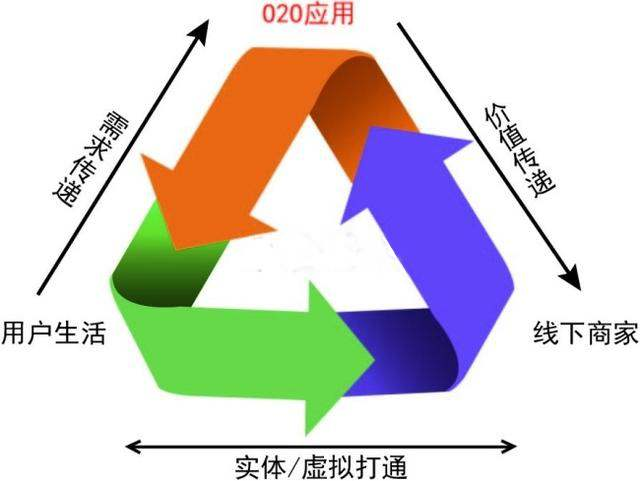
\includegraphics[width=9cm]{fig/22}
	\caption{营销模式图}
\end{figure}
虽然我们采取的是线上线下相结合的传统营销模式,但针对用户需求和用户体验,要做到精准营销,又会有不同的侧重点。随着互联网的快速发展,电子商务模式除了原有的B2B,C2B,C2C,商业模式之外,一种新型的消费模式C2B已快速在市场上发展起来。我们采用C2B营销模式即离线商务模式,利用线上营销线上购买带动线下经营和线下消费。通过打折、提供信息、服务预订等方式,把线下商店的消息推送给互联网用户,从而将他们转换为自己的线下客户。



\subsubsection{线下渠道}
线下实体渠道主要是通过线下与超市平台达成合作,在本地和全球范围开发优质供应商,以场景定位的方式销售来自世界各个国家和地区的食材,并确保食材质量,按时配送。我们以平台为中心,打造平台、超市双方合作的营销平台。

\begin{itemize}
	\item 平台层
	
	我们平台会根据用户的喜好或者是用户每餐的饮食热量需求,提供合理搭配的推荐菜品,并给出相应的原材料采购建议,以方便用户进行自己的健康饮食计划,而不会因为原材料采购问题而再次放弃。
	
	\item 超市层
	
	我们平台的最终目的是建立一个与超市达成合作的电商平台,我们生成的菜品原材料采购建议可以直接与超市进行对接,采购建议可以在平台上直接生成订单在超市内部进行选购、称重、打包、配送。为用户提供新鲜的食材和灵活的订购方式,改变消费者食品采购方式。
	
	\item 用户层 
	
	“食刻Diet”小程序通过板块的划分让用户可以个性化(每个人的需求和个人情况不同我们通过营养学的计算公式计算个人的热量需求和热量消耗)从而为用户安排每餐热量的分配或是菜谱的建议,用户可以根据的喜好或者是对每餐的饮食热量需求,在每餐的推荐安排上进行切换,也可以根据自己的需求和偏好对系统生成的采购订单原材料种类、数量进行修改,从而在线上下单,帮助用户省去亲自到超市进行挑选称重的麻烦,直接配送到家。用户也可以自行选择配送日期和地点,并可以在距离下次配送5天以前随时修改、暂停或取消订购。 
	
\end{itemize}

\subsubsection{线上渠道}
\begin{itemize}
	\item 新媒体营销 
	
	本平台会利用微信、微博、B站等新媒体的平台以及Keep、Fit、即刻健身等运动减脂健身平台,开展推广营销活动。利用新媒体引导大家关注健康饮食、功能性饮食的同时推广我们的品牌,利用微博博主、微信公众号推送、B站博主等推广本小程序的内容、功能,并给用户发放优惠券等推广我们的产品终端。
	
	此外,公司也会在新媒体上设立相关的客服工作人员,与客户进行一对一的沟通交流,及时解决客户的问题,为用户提供高质量的售后服务,从而使得公司的用户群体的种类更广。同时,我们也会要保持固定的更新频率,对菜单进行更新,给用户不同的体验。 
	
	\item 搜索推广 
	
	搜索引擎推广是覆盖面广、针对性强、按效果付费且推广管理体系较为专业的推广方式,所以公司会在百度、google等网站进行搜索推广。我们将主要采取竞价搜索的方式,对:健康饮食、减脂、健身、烹饪、美食等关键词进行搜索排名提高,以此来提升小程序的访问量,提高公司的知名度。 
	
	\item 与相关APP互利合作 
	“食刻有限责任公司”将积极与Keep、Fit等影响力较高的健身减脂APP进行交流合作,在引入期通过价格竞标购买其广告版面,宣传营销,当平台进入成长期或成熟期之后逐步开展与各大知名新媒体平台的互惠合作,通过互置链接,互推产品等方式,共享客户群,扩大用户数额,达到互利共赢。 
	
	\item 开展短视频营销 
	以目前较火的短视频行业为切入点,通过制作一些精美引流的烹饪短视频在抖音、快手、火山小视频等短视频应用上定期常态化投放,相对于静态宣传视频宣传更具有感染力,容易引其客户应用冲动。在制作视频的同时要将“食刻有限责任公司”旗下主推产品“食刻Diet”的小程序特点,平台内容积极融入进去,但也要避免过度商业化引起观众方案,力求达到趣味性、商业性、关注度等方面的有机结合统一。
\end{itemize}

%-----------%
\subsection{网红IP式营销}
\subsubsection{网红经济模式}

在互联网不断推陈出新的浪潮下,网红经济这种新生代模式,对电商的整体流量及运营都产生了巨大的影响,不少互联网巨头以及中小企业的电商平台,都开始借助网红经济的优势为平台带货,在营销和变现这方面,网红可以算是专家。网红的经济变现模式基本上都是遵循:打造旗帜鲜明的IP——吸精准粉——实现流量变现这个流程。

我们在推广营销平台的过程中,充分适应现下的网红经济模式,依托互联网特别是移动互联网传播及其社交平台推广,通过大量聚集社会关注度,形成庞大的粉丝和定向营销市场,打造专属的网红IP,并根据公司产品特点设计了IP拟人化卡通形象-时刻馋猫(如图\ref{IP}),吸引更多的流量、用户群体。但“食刻Diet”与淘宝等电商平台存在一定差异。淘宝等平台更趋于商品销售,把流量变现成为商品购买者。而“食刻Diet”更多的是服务型定位,把流量变现为平台固定用户群体,而不是向用户推销商品。

\begin{figure}[H]
	\centering
	\includegraphics[width=7cm]{fig/IP}
	\caption{时刻馋猫-IP卡通形象}\label{IP}
\end{figure}

\subsubsection{流量的积累与变现}

“食刻Diet”的网红IP营销模式,是通过微博、微信、抖音等这种更偏向社交和娱乐化的新媒体平台去接触潜在用户群体,用评论和转发的形式受众可以拥有更多互动,以IP拟人化卡通形象-时刻馋猫增强趣味性,吸引更广大用户群体的关注。熟悉的新媒体平台投放,用户对“食刻 Diet的认知也会别有印象,增加用户粘性。在品牌内容营销的过程中,各个平台互相关联,打破信息孤岛,通过不断的分享,形成了传播矩阵,以微博,微信等为主导,其他媒体平台做辅助,进行营销传播,达到最终的营销目的。

在内容营销传播方面,本公司在抖音、微博、B站、公众号平台运营自己的官方号。在初期进行一定的流量积累,吸引关注度,暂时不进行任何的广告类宣传,不急于变现。而当平台运营达到稳定阶段,拥有一定的个用户关注度时,我们将实现商业变现,达到最终营销目的。

此外,本公司将拍摄一些古风美食制作视频、网红食物的制作教程、以及吃播视频,并发布一些饮食知识科普信息等等,精准吸引较为关注饮食、烹饪的流量,发展潜在用户。在运营过程中,也保持与积累流量受众的互动性,增强流量的黏着性。并且可以通过固粉式营业,对用户进行深入了解,更有针对性地调整平台运营方案。

在关注度趋于稳固后,将视频逐步植入平台,比如在某个烹饪制作视频插入平台使用片段,展示平台带来的良好用户体验。让用户产生好奇,主动发掘。逐步向积累地流量受众推荐“食刻Diet”平台。 

这些运营的官方号仍旧要持续运营,发布内容依旧需要保持较高的质量,进而维持受众的黏着性,并吸引更多的新流量。打造出平台专属的网络IP,不断为平台引流,输送更多用户群体。



%-----------%
\subsection{阶段营销}

\subsubsection{引入期}

在该阶段“食刻有限责任公司”的产品较新,关注的人会比较少,很多用户缺乏对我们产品的了解。当然,产品本身可能也不够完善,存在一定的不足之处。因此,在这一阶段,我们将通过调查研究进一步了解市场需求,针对用户的痛点进行详细地分析,同时在宣传上的重点主要体现在让用户了解到我们的企业价值所在,突出“食刻Diet”产品的差异性,在宣传方式上,一方面利用资金优势开展线下线上的大力推广,另一方面积极寻找超市、相关APP、专业健身人士以及社会上的合作伙伴,进行资源互换、双向交流,提高品牌知名度。

在用户服务上,我们应该坚持“顾客是核心”,在激烈的市场竞争中,抓住顾客的实际需求,以服务为重点,尽可能的为用户提供专业的推荐方案,完成“食刻Diet”小程序界面不断改进、不断优化,功能不断更新、丰富的过程,有利于我们公司的口碑传播。

\subsubsection{发展期}

经过前期的一系列摸索,在发展期本公司产品“食刻Diet”小程序的风格、整体界面、功能已经基本确定,用户增长也相应进入了一个起速的阶段,这时用户属性会大致分为两个主要部分。前期忠实用户群体以及后期新参与进来的用户群体。

对于刚刚开始使用“食刻Diet”小程序的客户,要抓住时机,利用平台自身特点为用户提供良好的服务,让用户感到“食刻Diet”小程序的方便快捷。与此同时,我们也会利用“食刻Diet”的增长潜力与更多的商业伙伴达成合作,加大宣传力度,增加营销费用,争取增加产品曝光量。

而面对忠实的老用户群体要对他们发放一部分既得利益,通过线上放送优惠卷、解锁新菜品等活动的开展,让他们产生优越感,增加他们的使用频率,使他们形成一个“死忠”粉丝团体,同时在未来也可能是平台“最佳最坚固的传播圈子”,推荐给身边的家人、朋友以及同学同事使用。

\subsubsection{成熟期}
进入成熟期之后市场会逐渐趋于饱和,虽然用户会保持一定速度的增长,但增长速度明显放缓。在这一阶段,“食刻有限责任公司”在营销上会更加注重用户分流,会对不同的用户群体进行市场细分,开展适合其属性的营销策略,维持客户粘度。

一方面,要不断注意新机会的出现,在营销上以“新”为主,譬如适时改变平台风格、界面布局等,让客户产生新的视觉感受以及使用体验,而不至于产生审美疲劳而导致用户迁移。

另一方面,平台会开展一些新的活动,例如:满减活动、促销活动、免费提供健身餐搭配等等,让用户对“食刻Diet”产生寄托,培养附属感、依赖感。

%-------------------%
\subsection{整合营销}
“食刻有限责任公司”旗下主推产品“食刻Diet”在整体营销上将以罗伯特·劳特朋在1990年提出的4C 理论为基础,即围绕瞄准顾客需求(Consumer),研究顾客所愿意支付的成本(Cost),考虑顾客使用的便利性(Convenience),与顾客进行沟通(Communication)来制定更加完整的营销战略,以顾客为中心,以顾客的需求为导向。整体营销战略的总体目的是吸引更多的用户,增加用户粘性,维持用户忠诚度。首先应该把追求用户满意放在第一位,其次是努力降低用户的使用成本,然后要充分注意到用户使用过程中的便利性,而不是从平台的角度来决定销售营销策略,最后还应以用户为中心实施有效的营销沟通。

\begin{figure}[!htb]
	\centering
	\includegraphics[width=12cm]{fig/24}
	\caption{4C营销策略图}
\end{figure}


\subsubsection{顾客需求策略}

以顾客为核心,注重顾客体验式消费,提供高品质、便利性的服务。“食刻Diet”高度关注顾客对于“健康、健身、减脂、方便”的需求,为用户提供个性化菜谱推荐,提供由营养学家和厨师团队制定的定期更新的健康食谱,挑选容易保鲜的食材,并配以快速便捷的烹饪步骤,从而保证用户居家烹饪的良好体验。顾客在线下单,超市选购、称重、打包,即刻配送,让用户每一天都能享受新鲜的食材,健康美味的菜肴。满足用户期望方便快捷地享受健康地居家烹饪的需求。

在马斯洛的需求层次论看来,人的需求一共分为五个层次,分别是生理需求、安全需求、社交需求、尊重需求和自我实现需求,基于这五种层次,我们从用户的角度出发,进行产品设计和营销。

\begin{figure}[!htb]
	\centering
	\includegraphics[width=10cm]{fig/23}
	\caption{马斯特洛需求层次理论}
\end{figure}

\subsubsection{成本策略}
“食刻Diet”的最终目的就是作为一个与超市进行合作的电商平台,我们生成的原材料采购建议可以直接与超市进行对接,一定程度上降低了人工成本。线下超市同时作为物流中转中心,提供配送服务(与美团达成合作,使用美团的骑手资源),配送消费成本低。

“食刻Diet”平台,小程序注册免费,提供的推荐菜品以及菜品的制作方法大部分采取免费模式,以免费策略来吸引用户,减少外界视“食刻Diet”过度商业化的标签,培养客户对“食刻Diet”平台的信任感,归属感。
 
在付费服务方面,具体分为两类: 

(一)普通用户可升级为会员,会员用户将享受更多推荐菜品以及健身餐的搭配方案。

(二)用户若线上下单,需要根据自己与超市的距离远近支付一定的配送费。

\subsubsection{顾客使用便利性}

“食刻Diet”实现了线上线下完全融合。一方面,所有线下的商品与服务都可以在线上操作,帮助用户节省下进入超市挑选、称重的麻烦,可以直接采用配送外卖的形式,在距离自己最近的一家超市下单后配送到家。另一方面,“食刻Diet”通过与营养学家和厨师团队的合作,提供从食谱研制到食材供应的全套居家烹饪解决方案,使用户可以足不出户就享受到专业人士的健身餐搭配方案或者是美味的菜品。

此外,在小程序的设计上,简单好用是我们的设计宗旨之一,这也是我们对外推广的重点之一,质量至上就是要站在用户的角度,提升用户使用观感,简化操作流程,最大限度的提升用户操作的便利性,通过以质引量,吸引客户,增加客户粘性。

“食刻Diet”更多的考虑用户的方便,通过好的售前、售中和售后服务来让用户在使用的同时,也享受到了便利。便利是客户价值不可或缺的一部分。

\subsubsection{顾客沟通策略}
在对外营销上,“食刻Diet”会加强注重与客户之间的沟通交流,设立相关的客服工作人员,与客户进行一对一的沟通交流,及时解决客户使用小程序的问题,为用户提供高质量的售后服务。沟通一方面改善客户的应用体验,加深顾客对品牌的认知度,加强客户粘性;另一方面在与用户的沟通交流中,我们也会积极自检发现平台本身存在的问题,着手改善,提升平台自身实力,为吸引用户提供更大的势能储备。

“食刻Diet”增进与用户的沟通,建立基于共同利益的新型平台-用户关系。这不再是平台单向的促销和劝导用户,而是在双方的沟通中找到能同时实现各自目标的通途。

\newpage
%---------------------------------------------------------------------------------------------%
\section{财务分析}
\subsection{财务管理制度总则}
为适应“食刻有限责任公司”发展需要,建立现代化企业制度,以及建立健全财务管理体系,充分发挥财务在公司经营管理和提高经济效益中的作用,使公司做到资金合理分配及有效运用,规范公司财务行为,加强财务管理和经济核算,以不断提高经济效益,结合我公司特有的融资及盈利模式制定了本制度。本制度根据中华人民共和国颁发的《企业会计准则》和《企业财务通则》制订,遵循公司管理制度、发展目标和管理要求,并结合本公司的实际情况进行细化。
 
“食刻有限责任公司”实行总经理领导下,由财务部总监与财务经理共同负责制财务管理体制,统一安排部署会计核算,负责资金的筹集、使用,进行财务管理。各部门财务实行部门经理和财务专员共同负责制。

“食刻有限责任公司”实行全面预算管理,财务管理应做到规范性、计划性、效益性。要做好各项财务收支计划、监督、核算、分析和考核工作。以业务预算、资本预算为基础,以经营利润为目标,从而合理配置资源,实现资源最大化。

“食刻有限责任公司”财务部分应加强财务管理和会计核算基础工作,以提高会计核算与财务管理质量,在经营活动中产生的非正常这就资产损耗,都应做好完整原始记录。

“食刻有限责任公司”财务部门应定期进行财产检查,加强财务核算电算化管理,以保证会计信息的及时性、准确性、安全性。公司内部各部门根据管理要求和实际情况,建立部门财务专员制度,进行在公司财务部门监督下的独立核算和业绩考评。

本公司将严格执行财政部 2011年颁布的《企业会计准则》及其应用指南,以自然年度作为会计年度,即每年 1 月 1 日至 12 月 31 日。本财务管理制度适用于本公司所有部门。本财务管理制度由公司财务部门负责解释。 

%------------%
\subsection{相关会计事项}
\subsubsection{会计假设}
会计假设亦称会计的前提,是指在特定的经济环境中,根据以往的会计的实践和理论,对会计领域中尚未肯定的事项所做出的合乎情理的假说或设想。针对本公司的财务结构特点,结合《企业会计准则》及其应用指南,主要基于以下四个基本假设:
\begin{itemize}
	\item[*] 会计主体假设
	
	会计主体是指会计工作服务的特定单位,是企业会计确认、计量和报告的空间范围。会计主体假设的重要意义在于界定了权益的范围,规定了会计核算的空间。
	
	\item[*] 持续经营假设
	 
	持续经营,是指会计主体的生产经营活动将无期限持续下去,在可以预见的将来不会倒闭进行结算。在持续经营前提下,会计确认、计量和报告应当以企业持续、正常的生产经营活动为前提。持续经营是对企业经营过程的描述,是一个无限的时间段概念。本公司同样适用于持续经营假设。
	
	\item[*] 分期假设
	
	会计分期假设规定了会计对象的时间界限,将企业连续不断的经营活动分割 为若干较短时期,以便提供会计信息,是正确计算收入、费用和损益的前提。如 上所述,我公司按照《企业会计准则》规定,以自然年度作为会计年度,即公历 1 月 1 日至 12 月 31 日为会计核算的时间区间。 

	\item[*] 货币计量假设 
	
	货币计量是指企业在会计核算中要以货币为统一的主要的计量单位,记录和反映企业生产经营过程和经营成果。货币计量假设规定了会计的计量手段,指出企业的生产经营活动及其成果可以通过货币反映。
	
\end{itemize}

\begin{figure}[!htb]
	\centering
	\includegraphics[width=10cm]{fig/25}
	\caption{会计基本假设}
\end{figure}


\subsubsection{税率}
根据国家相关税收政策与税收法规,“食刻有限责任公司”暂拟服从以下税率: 
国务院批准的高新技术产业开发区内的高新技术企业,减按 15\%的税率征收所得税;新办的高新技术企业自投产年度起免征 2 年企业所得税(94 年财税字第 001号)。因此企业开办后从获利年度起两年内不征所得税,接下来的年份按 
15\%的税率征收。 

营业税率为 7\%,其他税务支出为城市维护建设税,按营业税额的 7%计算;
教育费附加,为营业税额的3\%。 

公司为一般纳税人。运营涉及实物流转,因此考虑增值税,税率为17\%;
企业贴现率按 10\%计算。

\subsubsection{固定资产折旧 }
固定资产折旧采用直线折旧法。本公司主要的固定资产为服务器,服务器属于电子设备类,电子设备使用期为 3 年,因此固定资产折旧 计算时使用期为 3 年。考虑服务器的更新换代速度,达到使用年限后其残值假设 为 0。固定资产购入当年不计提折旧。
\subsubsection{无形资产摊销 }
无形资产分 5 年摊销,使用寿命有限的无形资产,其残值应当视为零。 但下列情况除外: 

(1)有第三方承诺在无形资产使用寿命结束时购买该无形资产; 

(2)可以根据市场活跃得到预计残值信息,并且该市场在无形资产使用寿 命结束时很可能存在。


\subsubsection{利润分配政策}

利润分配,是将企业实现的净利润,按照国家财务制度规定的分配形式和分 配顺序分配给投资者,是投资者持股收入的主要来源。

分配顺序按以下进行:  

按税后利润的10\%提取法定盈余公积金;  

按税后利润的 5\%提取法定盈余公益金; 

为对风险投资进行回报,本公司将从开始获利的第二年起,按公司净利润的10\%用于分红,按各年公司的具体盈利情况而定。

%-------%
\subsection{融资方案} 
融资是指为支付超过现金的购货款而采取的货币交易手段,或为取得资产而 集资所采取的货币手段。融资通常是指货币资金的持有者和需求者之间直接或间 接地进行资金融通的活动。融资为企业的投资提供了资金保障,为企业发展壮大 提供可能。
tion{}

\subsubsection{初期阶段}

\begin{enumerate}
	\item [(1)]“食刻有限责任公司”创始人合伙出资 350 万,并获得相应股份 
	
	\item[(2)]向金融机构借贷 50 万,年利率为 6.4% 
	
	\item[(3)]引入风险投资公司入股,投资 300 万
	
\end{enumerate}
公司注册资本约 700 万元。


\subsubsection{中期阶段}

经过2-3年的发展, 当“食刻有限责任公司”渡过了引入期,已经有一定市场,企业实体趋于成熟,预测用户数将面临爆发式的增长。此时,电子商务平台需要增加更多的功能,宣传投入力度将继续扩大。可以进行第二阶段融资,计划融资850万资金,充分发挥企业线上及线下的全部优势。

\subsubsection{上市阶段}

经过中期的发展,“食刻有限责任公司”已占有了可观市场份额,此时公司已经很具发展潜力和吸引力,计划融资2-3亿。 


%----------%
\subsection{财务资料预测}

\subsubsection{前期投入及费用预测}

\begin{figure}[!htb]
	\centering
	\includegraphics[width=10cm]{fig/26}
	\caption{前期投入费用预测表}
\end{figure}


\subsubsection{预计利润表(5年)}
\begin{figure}[!htb]
	\centering
	\includegraphics[width=10cm]{fig/27}
	\caption{利润表(5年)}
\end{figure}

\subsubsection{收入预测}

“食刻有限责任公司”收主要有三大组成部分:销售收入、广告收入、增值业务收入。

\begin{itemize}
	\item 销售收入
	
	销售收入主要来自于小程序会员费用、套餐费用以及服务费。
	\begin{figure}[!htb]
		\centering
		\includegraphics[width=10cm]{fig/28}
	\end{figure}
	
	\item 广告收入
	\begin{figure}[!htb]
		\centering
		\includegraphics[width=10cm]{fig/29}
	\end{figure}	
	
	\item 商家利润分成收入
	\begin{figure}[!htb]
		\centering
		\includegraphics[width=10cm]{fig/30}
	\end{figure}
	
\end{itemize}

%--------------%
\subsection{投资回报分析}
\subsubsection{投资回收期}
投资回收期是指从项目的投建之日起,用项目所得的净收益偿还原始投资所
需要的年限。投资回收期越短说明投资风险越小。 
静态投资回收期=(累计净现金流量出现正值的年数-1)+上一年累计净现金
流量的绝对值/出现正值年份净现金流量  
由此公式计算可得,投资回收期较短,说明在财务上,该方案可行。

\subsubsection{投资净现值}

计财务净现值 $NPV=\sum(CI−CO)t (1+IC)t $  \ 式中:$t$ 为计算年份数,$(CI − 
CO )t$ 为第$ t $年的净现金流量,$IC $为折现率。  
计算得 $NPV>0$ 
因此,投资报酬率将超过投资者要求的报酬率,该方案可行。

%-----------%
\subsection{退出机制}
风险投资的本性是追求高回报的,这种回报不可能像传统投资一样主要从投资项目利润中得到,而是依赖于在这种“投入—回收—再投入”的不断循环中实现的自身价值增值。所以,风险投资赖以生存的根本在于资本的高度周期流动,流动性的存在构筑了资本退出的有效渠道,使资本在不断循环中实现增值,吸引社会资本加入风险投资行列。一个顺畅的退出机制也是扩大风险投资来源的关键,这就从源头上保证了资本循环的良性运作。可以说,退出机制是风险资本循环流动的中心环节。

退风险投资退出途径一般有:一、股份上市;二、兼并与收购;三、 股权回购;四、破产或清算。

一个理性的企业家在进入某一行业时一定会考虑退出的情形,如果一个产业退出的门槛太高,那么该产业的垄断程度也会越高,在企业万不得已要退出时,我们要尽最大努力将损失减到最小。“食刻有限责任公司”结合自身运营条件,经过综合考虑,撤出机制以实现预期资本获利目标为标志,撤出的方式有四种:股份上市、兼并与收购、股份回购和破产或清算,本公司将根据实际运营情况适时采取合理的方式。

\subsubsection{股份上市}

公开上市是风险投资最佳退出途径,它是指将风险企业改组为上市公司,风险投资的股份通过资本市场第一次向公众发行,从而实现投资回收和资本增值。 
 
若“食刻有限责任公司”运营顺利,成功进入市场,将选择在证券市场上市,上市有两种方式:IPO (首次公开发行股票)和买壳上市。IPO 具有募集资金、流通性好、树立名声、 回报个人和风险投入的优点,是风险投资最佳退出途径,是风险投资家追求的目标。另一方面,买壳上市也是很好的上市方法,门槛低,风险小,前提是有很好 的“壳公司”、良好的融资渠道等条件。采用IPO上市或者是买壳上市要根据公司后期发展情况决定。当“食刻有限责任公司”发展到初具规模、有很强的生命力的时候,本公司将采取申请上市的途径实现融资。

\subsubsection{兼并与收购 }

兼并收购是资本运营的重要形式,由于买方无需支付现金,因此交易找寻买家,交易技巧性和灵活性大。风险资本选择并购方式退出,最常用的操作途径有三种:

\begin{itemize}
	\item[*] 直接收购
	
	收购者用现金直接收购买目标企业的股份,这是小型高科技公司被收购的主要方式,并不适合本公司。
	
	\item[*]杠杆式收购
	
	收购者没有足够的资金来收购目标企业,它是以贷款或发行债务证券的方式 来购买目标企业的股份,再利用收购回来公司所能提供的现金流来支付该项贷款 的利息。
	
	\item[*]管理收购
	
	管理收购指的是企业内部管理层以杠杆式收购的方式贷款买公司的大部分股份并成为收购者。
	
\end{itemize}

如果“食刻有限责任公司”发展没能达到期望的要求,实力不够强,但又因为具有独特的技术、良好的前景,其他的企业或投资者就可能对它感兴趣,把它兼并收购下来。从公司发展来看,被兼并后本公司可能不复存在或名存实亡,此时股东可以借机抽身,不但能收回全部投资,还能取得可观的收益。当然,如果公司是因为发展受阻自己寻求兼并例外。

%-------------------%
\subsection{股权回购}

所谓股权回购,风险企业以现金的形式向投资基金回购本公司股权。风险投资者可以拿到现金(或可流通证券),而不仅仅是一种期权,可以迅速地从风险企业中撤出;而且股权回购只涉及风险企业与风险投资方两方面的当事人,产权关系明晰,操作简便易行;并且可以将外部股权全部内部化,使风险企业保持充分的独立性,并拥有足够的资本进行保值增值。

根据签订的投资协议设定,当投资期满后,如果创业公司无法上市或股权无法转售给其他公司的情况下,创业公司可以自有资金回购风投公司的股权。这种退出方式一方面解决了创业公司阶段性资金需求,另一方面又满足了创业者的对公司控股权的要求。 

根据“食刻有限责任公司”的运营情况分析,上市之后,公司可利用盈余所得后的积累资金(即自有资金)或债务融资以一定的价格购回公司本身已经发行在外的普通股,将其作为库藏股或进行注销,以达到减资或调整股本结构的目的,同时也保护了中小股东的权益。

%----------------%
\subsection{破产或清算}

风险投资的高风险反应在高比例的投资失败上,相当大部分的风险投资不很成功,且越是处于早期投资的风险的风险投资失败率越高。

被投资的企业因经营不善等原因宣布破产清算,这是风险投资家最不愿意看到的结果。但高风险的特点决定了每一家风险投资公司都要面对完全失败的投资项目。

清算方式的退出是痛苦的,但在很多情况下是一种必须采取的断然措施。如果企业失去了发展可能性或者成长速度太慢,不能给予预期的高回报,就应果断地撤出资金,宣布公司解散,将能收回的资金用于下一投资循环。

理性的公司应该在其经营管理发生困难没有发展可能是及时宣布解散,如果决策以及对形势的预测错误导致了破产,那么要尽最大努力偿还债务,诚信是商业成功之本,留下好的口碑可以为东山再起打下良好的基础。

综合上述四种风险退出机制的比较,四种方式都可能被公司采用。若“食刻有限责任公司”发展壮大一定程度后,成功上市,那么“公开上市”是公司的最佳退出的方式;第四种破产清算的方式退出是企业建设者和经营者都不愿意的选择的方式。但是在企业经营状况恶化的情况下必须断然采用措施。选择退出方式时,要根据“食刻有限责任公司”的发展情况和时机而定,采取最有利的风险退出机制。

\newpage
%---------------------------------------------------------------------------------------------%
\section{关键的风险和问题}
%-------------------%	
\subsection{技术风险及对策}
\subsubsection{技术开发风险及对策}

\begin{itemize}
	\item \textbf{技术开发风险:}
	
	公司由大学生创业,将更多地从相关高校或合作企业中寻找相关专业技术人员,以确保开发的顺利进行。但这也带来了一个问题,大学生的开发经验并不充足,对整体架构的把握不到位,这有可能造成后期维护困难等问题。公司初期容易存在运营金额不足的问题,这也会在一定程度上造成人员流动性大,技术开发团队工作量大等问题,容易导致小程序开发工作的拖延。
	
	\item \textbf{技术开发风险的对策:}
	
	开发后期也会聘请专门架构师进行把关和规划,加大技术投资以保证开发的顺利进行。同时,我们也会最大限度的保证开发团队的人员稳定性,避免开发人员满负荷工作,适当的扩大开发团队规模,防止因为部分开发人员的中途退出而导致程序开发受阻,尽可能保证按部就班地进行。
	
\end{itemize}

\subsubsection{信息安全风险及对策}

\begin{itemize}
	\item \textbf{信息安全风险:}
	
	在信息系统中存储、传递用户信息时,用户信息可能被恶意窃取、利用和窜改,或者在信息处理过程中可能产生丢失或被破坏等类似的安全问题。如用户在支付订单时可能会遇到支付失败或者扣除金额但却没有显示等问题;用户可能在接受订单配送时有被泄露位置信息的风险等。
	
	\item \textbf{信息安全风险的对策:}
	
	面对网站运行的安全性风险存在,我们要加强技术开发,利用信息加密技术和防火墙技术等更好的保证用户的隐私;选择值得信赖的第三方支付合作伙伴,明确权责关系,适当监督。只有做到了信息保密和信息不被恶意窜改,才能保证在平台上交易的双方的切身利益,提高用户对公司的信任度。
	
\end{itemize}
%-------------------%	
\subsection{市场风险及对策}
\subsubsection{用户市场风险及对策}

\begin{itemize}
	\item \textbf{用户市场风险:}
	
	如今市场上也有一些关于生鲜配送的电子商务平台,也不乏专攻健康饮食指导的用户专栏,他们已有了一定的客户资源积累知识分享,用户对已有网站的依赖性对我们造成一定的影响,我们如何在现有的基础上争夺用户,提高食刻 Diet的市场占有率是当下需要重点考虑的问题。
	
	\item \textbf{用户市场风险的对策:}
	
	发挥食刻 Diet自身商业模式优势,打造集健康饮食搭配和菜谱原料配送为一体的最佳线上餐饮品牌,在用户购买、交流、分享的愉悦过程中提供相应增值服务和积分策略。充分发挥公司文化优势,让目标用户在这里找到归属感,对公司服务产生依赖性;我们也将借鉴当前线上餐饮配送龙头企业,以期获得更好的发展。
	
\end{itemize}
\subsubsection{原料市场风险及对策}

\begin{itemize}
	\item \textbf{原料市场风险:}
	
	用户一键式采购菜谱原料,食刻 Diet提供食材配送服务,这也就把需要本公司承担起监督原料供应商的责任。如果我们不能按时按需提供用户所需食材或不能给用户提供让她们满意的食材,久而久之,用户会失去对公司的信任和继续购物的热情,公司最终会有破产风险。
	
	\item \textbf{原料市场风险的对策:}
	
	建立大数据库,由公司联系配送超市应对原料供应情况并及时统计,同步原料更新等信息;加强对超市配送食材的监管,保证食材的安全性;加强与配送平台的联系,最大程度保证送到用户手中的食材新鲜度。
	
\end{itemize}
\subsubsection{配送方案风险及对策}

\begin{itemize}
	\item \textbf{配送方案风险:}
	
	在保证食材新鲜度方面,配送是一个不可忽视的重要环节。配送时间过长会导致食材不新鲜等问题产生;而过于频繁的派送又会增加成本,不利于公司的长久经营。因此,选择一个合适的配送方案至关重要。
	
	\item \textbf{配送方案风险的对策:}
	
	在公司成立初期,我们选择与外卖配送平台合作,按单给予平台骑手酬劳,这样既能保证配送能及时到达用户身边,又能保证公司合理运转。当用户数量达到一定规模之后,公司会逐步开展自行配送业务,自行招聘骑手开展配送,这样可以让配送更加方便快捷,增强用户的体验感。
	
\end{itemize}
\subsubsection{推广风险及对策}

\begin{itemize}
	\item \textbf{推广风险:}
	
	在公司发展初期,缺乏知名度,为了在第三方平台上推广需要大量投资,而且公司建立初期也存在缺乏合作方和客户的信任的问题,因此对于交涉超市加入食材配送合作也会面临一定的困难。同时,还存在被某些已经存在的拥有部分类似功能的产品模仿并被其他公司追赶的风险。
	
	\item \textbf{推广风险的对策:}
	
	在进行市场推广之前,进行充分的市场调研,保持对市场情况的敏锐的分析,准确把握市场动向。寻求大量资本,利用成立初期的优势,逐步引导各种平台加入,让用户尝到红利,让第三方平台赚的利益,推广也就水到渠成。差异化竞争确立市场地位。作为初创公司,再找准市场定位的基础上,利用先入者的优势快速建立自己的市场地位,顺势推广扩大。
	
\end{itemize}
%-------------------%	
\subsection{财务风险及对策}

\begin{itemize}
	\item \textbf{财务风险:}
	
	公司现有的融资渠道主要是合伙人投资和银行贷款,由于启动资金较为庞大,且公司运营初期可能会出现一些决策失误造成资金亏损等,资金链可能会出现不同程度的问题。另外,风险资本具备一定的流动性,周转期一般为3—5年,这也是公司成长最关键也是最迅速的时期,为储蓄核心竞争力、积累用户、培养用户习惯,可能会有一段时间的亏损期。这更加需要充足的资金保证,否则。资金链一旦断裂,公司将面临各项服务业务无法开展、客户流失、下游供应链断裂等问题,甚至会走向破产边缘。
	
	\item \textbf{财务风险的对策:}
	
	公司应增强风险意识,提高决策水平。合理规划公司的运营,脚踏实地运作。健全公司机制,保障投资人的利益,增强投资人的信心。同时完善财务管理系统,夯实基础性工作,努力减少一切可以避免的损失。建立有效的风险预警系统,对公司内部经营状况与外部市场环境进行定期评估,预先发现公司可能面临的风险并对风险性质、波及程度大小等进行评估。
	
\end{itemize}
%-------------------%	
\subsection{人才资源风险及对策}

\begin{itemize}
	\item \textbf{人才资源风险:}
	
	公司初始创立成员均为在校大学生,缺少经验,同时由于公司的服务涉及虚体、实体、网上购物及线下物流等多个方面,部门的设立不是一件容易的事情。由于初期资金等问题,公司初期对优秀员工的吸引力不足,员工薪酬可能也会受到公司效益的影响。而小程序建设和维护都需要先进的开发技术和多方面的开发人才,如何能在小程序运营初期通过招聘各类人才从而拥有一支可靠的技术和管理团队是对我们这个初创公司的考验。
	
	\item \textbf{人才资源风险的对策:}
	
	经营初期,将一部分资金用于聘请有电子商务领域经验的员工,充分利用他们的阅历和才能,为我公司电子商务平台的投入市场提供员工培训,力求少出差错。采取网络,媒体,平面的营销模式扩大企业的知名度,树立企业的品牌,把广阔的晋升空间、友好的上下级关系、倡导轻松搞笑的工作氛围作为我们创业公司的优势进行宣传,以吸引更多的人才加入我们的公司;对公司员工进行必要的培训,以提高员工的业务水平。从长期来看,塑造良好的企业文化,树立正能量的价值观念,建立合理的奖惩机制,提高工作团队的进取心和活力,营造和谐上进的工作氛围,加强公司凝聚力和创造。
	
\end{itemize}

%-------------------%	
\subsection{法律风险及对策}

\begin{itemize}
	\item \textbf{法律风险:}
	
	在我公司电子商务业务运营初期,对于电商经营等的规定不够熟悉,容易在某些地方由于疏忽出现违规内容。如在公司内部,对于员工薪资、招聘等问题处理不慎所引发的法律问题;因为涉及到用户的个人信息,这些内容一旦泄露,可能会对网站产生不利影响,引起法律上的纠纷;公司在需要从各个领域中获取大量信息时,借鉴其他企业的经验,在此过程中,可能会涉及到侵权问题;公司在与其他企业在市场中容易产生引起不正当竞争、侵犯商誉等方面的法律问题。
	
	\item \textbf{法律风险的对策:}
	
	公司会加强对国家法律与相关政策的关注,聘请专业法律顾问不断完善电子商务市场的规范性并进行相关的指导,严格依照《劳动法》及《劳动合同法》处理公司内部劳动合同关系;及时对公司的创意申请专利,提升公司人员对知识产权的保护意识,避免侵权与被侵权的事件发生;通过《电子商务环境下的消费者保护准则》的相关规定来解决平台交易过程中发生的权益、法律等纠纷。
	
\end{itemize}



%---------------------------------------------------------------------------------------------%

\end{spacing}

\ClearShipoutPicture

\end{document}
